\documentclass[a4paper]{report}
\usepackage[T1]{fontenc}
\usepackage[swedish]{babel}
\usepackage{graphicx}
\usepackage{listings}
\usepackage{courier}
\usepackage{url}
\usepackage{float}
\usepackage[swedish]{varioref}
\usepackage{cite}
\usepackage{pdfpages}


%% Define a new 'leo' style for the package that will use a smaller font.
\makeatletter
\def\url@leostyle{%
  \@ifundefined{selectfont}{\def\UrlFont{\sf}}{\def\UrlFont{\small\ttfamily}}}
\makeatother
%% Now actually use the newly defined style.
\urlstyle{leo}

% Konfigurera utseende p� kodlistning
\lstset{
basicstyle=\small,
frame=lines,
postbreak=\space, 
breakindent=5pt,
breaklines,
xleftmargin=17pt,
framexleftmargin=17pt,
framexrightmargin=5pt,
framexbottommargin=4pt,
showstringspaces=false,
showspaces=false,
showtabs=false}

% Avstavningar
\hyphenation{XML-Http-Request}
\hyphenation{XML-Http-Request-objektet}
\hyphenation{web-server}
\hyphenation{web-servern}
\hyphenation{verktygs-program}
\hyphenation{verktygs-programmet}
\hyphenation{Java-Script}
\hyphenation{design-val}
\hyphenation{Design-val}
\hyphenation{l�nk-attribut}
\hyphenation{expedierings-objekt}


%\usepackage{color}
%\usepackage{xcolor}
%\usepackage{caption}
%\DeclareCaptionFont{white}{\color{white}}
%\DeclareCaptionFormat{listing}{\colorbox{gray}{\parbox{\textwidth}{#1#2#3}}}
%\captionsetup[lstlisting]{format=listing,labelfont=white,textfont=white}

\author{Steve Eriksson \\steer237@student.liu.se}
\title{Interaktiv visualisering av IP-n�tverk}
\date{Link�ping, \today} 

\begin{document}

\includepdf[pages=1]{idasidor/rapportframsida.pdf}

\includepdf[pages=1]{idasidor/rapportinsida.pdf}

%\maketitle

\pagenumbering{roman}

% Sammanfattning
\renewcommand{\abstractname}{Sammanfattning}
\begin{abstract}


Telenors svenska n�tverks�vervakning har utvecklat ett system f�r att
automatiskt generera n�tverkskartor i formatet SVG.
De har st�llt fr�gan om det g�r att g�ra dessa interaktiva och koppla
ihop dem med befintliga verktygsprogram.

Denna studie visar tekniker som kan anv�ndas f�r att utveckla ett system
som g�r SVG-baserade n�tverkskartor interaktiva i en webbl�sare.

Ett system baserat p� �ppen mjukvara och �ppna standarder utvecklas f�r att
visa hur teknikerna kan anv�ndas i praktiken.
Systemets arkitektur beskrivs i tre systemvyer.
N�tverkskartorna berikas med bindningar mellan h�ndelser i
webbl�saren och JavaScript-funktioner genom att transformera dem med XSLT.
Anv�ndargr�nssnittet utg�rs av SVG-objekt och JavaScript varifr�n det
g�r att asynkront anropa program p� en webbserver.

Studien avslutas med att utv�rdera systemet och ge f�rslag p� hur det
kan f�rb�ttras.

\end{abstract}


\tableofcontents
\listoffigures

% Svenska namn p� listningar
\renewcommand{\lstlistingname}{Listning}
\renewcommand{\lstlistlistingname}{Listningar}
\lstlistoflistings
\cleardoublepage % utan denna s� blir numreringen fel p� lol


% -------------------------------------------------------------------------------

\pagenumbering{arabic}
\chapter{Inledning}
% b�rja rapporten p� sida 1
\setcounter{page}{1}


\section{Bakgrund}
Telenor\cite{Telenor:om} i Sverige �r en av landets st�rsta leverant�rer av
kommunikation via mobil- och fast telefoni och �r
med k�pet av Bredbandsbolaget\cite{Bredbandsbolaget:om}, Sveriges n�st st�rsta
bredbandsleverant�r.

�vervakning och drift av Telenors IP- och mobiltelefonin�t i Sverige g�rs av Telenor
NOC\footnote{Network Operations Center} som �r bel�gen i Karlskoga.


�vervakning av n�tverken inneb�r att operat�rerna p� NOC tar emot larm fr�n
utrustning i dessa. Larmen kommer fr�n ett flertal olika leverant�rers
�vervakningssystem.
Operat�rerna tar �ven emot felanm�lningar via telefon, e-post och
�rendehanteringssystem.

Drift av n�tverken inneb�r att operat�rerna reagerar p� ovan n�mnda
larm och felanm�lningar och ansvarar f�r att defekter �tg�rdas
antingen av operat�ren sj�lv eller av en l�mplig tekniker.

De senaste �ren har det p� Telenor utvecklats flertal verktygsprogram f�r att
underl�tta operat�rernas dagliga arbete. Exempel p� dessa �r program som 
rapporterar hur m�nga kunder som �r inkopplade mot en viss n�tverksnod, hur 
m�nga noder det finns i en viss stad och hur m�nga av dem som �r kontaktbara.
De flesta av verktygsprogrammen �r UNIX-baserade program skrivna i programmeringsspr�ken  
Python, Perl och Bash och anropas via ett kommandoskal i UNIX.


\section{Existerande system}
\subsection*{Visualisering av IP-n�tverk} 
Telenor NOC har tillg�ng till n�tverkskartor som visar viktiga delar av IP-n�tverket.
Denna dokumentation utg�rs av dokument i olika filformat men gemensamt f�r dessa �r att de ej �r
dynamiska eller interaktiva; det saknas koppling mellan
element i dokumenten och motsvarande nod i IP-n�tverket.

\subsection*{Verktygsprogram}
N�tverkstekniker p� Telenor har utvecklat ett flertal verktygsprogram.
Dessa program �r skapta att k�ras i ett kommandoskal.
Varje program har egna f�ruts�ttningar och begr�nsningar vilket
betyder att anv�ndaren m�ste k�nna till vilka parametrar dessa
anv�nder och vilka krav som m�ste uppfyllas innan exekvering.


\section{Problem}
% Varf�r SVG? Vad �r problemet och varf�r vill man l�sa det s� h�r?
Telenors IP-n�tverk (forts�ttningsvis kallat n�tverket) �r omfattande och inneh�ller m�nga f�rbindelser
mellan noderna i det. Varje nod i n�tverket inneh�ller �tminstone ett tiotal
f�rbindelser, redundanta och icke redundanta, till andra noder.
Det �r d�rf�r sv�rt att bilda en mental modell �ver n�tverket.
N�r ett larm r�rande en bruten f�rbindelse eller att kontakten
f�rlorats med en nod i n�tverket inkommer till Telenor NOC �r det ofta
sv�rt att f�rst� hur problemet p�verkar n�tverket. 
Ett larm �r vanligtvis st�mplat med en identifierare f�r den aktuella noden och om
det r�r en f�rbindelse �ven ett indexnummer f�r den port f�rbindelsen
�r kopplad till.

% Ska detta st� h�r eller i motiveringen?
% Med en grafisk representation av n�tverket �r det l�ttare att f� en
% �vergripande 
% bild och direkt se vilka noder och f�rbindelser som p�verkas.

%arbetsfl�det, givet program, leta reda p� noden, var hittar man den?
% Ett vanligt arbetsfl�de p� Telenor NOC �r att givet en nod i n�tverket
% utf�ra ett verktygsprogram som till exempel listar antalet anslutna kunder f�r
% att kunna avg�ra hur omfattande en driftst�rning skulle vara om den
% aktuella noden skulle g� ner.
En vanlig uppgift p� Telenor NOC �r att uppskatta omfattningen av en
driftst�rning som uppst�r d� noder i n�tverket g�r ner. Driftst�rningar
kan uppst� via of�rutsedda h�ndelser som till exempel str�mavbrott
eller planerade arbeten, exempelvis uppgradering av en n�tverknods operativsystem.
Det finns p� Telenor NOC verktygsprogram som listar antalet anslutna
kunder till en nod men den listan inneh�ller ej information om
f�rbindelser till andra noder i n�tverket. Konfigurationen f�r varje
port i aktuell nod m�ste unders�kas f�r att avg�ra vilka andra noder den �r
ansluten till.


\section{Motivering}
En grafisk representation av n�tverket ger operat�rerna p� Telenor NOC en �vergripande bild �ver de
komplexa kopplingar som existerar mellan noder i n�tverket och de slipper skapa en
mental modell �ver dessa.
% Planjobb, l�ttare att se exakt p�verkan?

Telenor NOC har b�rjat unders�ka vilka m�jligheter det finns att visualisera delar av
n�tverket i ett SVG\footnote{Scalable Vector Graphics}-dokument och g�ra det interaktivt.
Man vill ocks� g�ra det m�jligt f�r en anv�ndare att anropa externa
program fr�n dokumentet.

Dokumentformatet SVG har valts av flera anledningar:

\begin{itemize}
\item SVG �r ett XML\footnote{Extensible Markup
    Language}-baserat dokumentformat och en fil i detta format �r
  tillg�nglig i klartext. 
  Dokumentet kan d�rf�r, till skillnad fr�n bin�ra format, enkelt analyseras av b�de
  m�nniskor och program. Data i dokumenten �r tillg�ngliga f�r
  framtida anv�ndare och utvecklare.

\item SVG �r ett dokumentformat f�r webben. SVG-dokument �r enkla att infoga i webbsidor och kan �ven
  anv�ndas sj�lvst�ndigt i en webbl�sare. Ett system utvecklat f�r att
  exekveras i en webbl�sare kr�ver ingen installation eller
  administration p� en anv�ndares dator vilket minskar arbetet med att
  underh�lla det. Det finns �ven m�jligheter att anv�nda tillg�ngliga
  webbtj�nster som till exempel Google Maps\footnote{En webbaserad karttj�nst.} f�r att �ka
  funktionaliteten i systemet.

\item SVG-specifikationen inneh�ller bindningar till 
  JavaScript och dokumenten kan d�rf�r g�ras interaktiva p� samma s�tt
  som webbsidor i HTML-format. Ett SVG-dokument kan anv�ndas b�de som
  en n�tverkskarta och som anv�ndargr�nssnitt i en webbaserad applikation.

\end{itemize}

% SVG har valts p� grund av att det �r en �ppen specifikation och
% baserat p� XML\footnote{Extensible Markup Language}.
% SVG-dokumentens kod �r tillg�nglig i klartext och kan d�rf�r
% till skillnad fr�n dokument i bin�ra format enkelt analyseras av b�de
% m�nniskor och program, vilket inneb�r att datan i dokumenten finns
% tillg�ngliga f�r framtida anv�ndare och utvecklare. 
% SVG-dokument �r enkla att infoga i webbsidor och kan �ven anv�ndas
% sj�lvst�ndigt i en webbl�sare. Ett system som �r utvecklat f�r att
% exekveras i en webbl�sare kr�ver ingen installation eller
% administration p� en anv�ndares dator vilket minskar arbetet med
% att underh�lla det.


\section{Syfte}
Syftet med detta arbete �r att utveckla ett prototypsystem som g�r n�tverkskartor i formatet SVG interaktiva.
Det ska vara m�jligt att via n�tverkskartorna anropa befintliga verktygsprogram.


\section{Avgr�nsningar}
Best�llaren har beslutat att anv�nda visualiseringsmjukvaran GraphViz f�r att generera 
n�tverkskartor i formatet SVG. Systemet beh�ver ej inneh�lla funktionalitet f�r att 
skapa konfigurationsfiler till GraphViz baserat p� befintlig topologi av 
n�tverket. Systemet beh�ver ej generera dessa n�tverkskartor.

Den del av systemet som exekveras p� klientsidan ska vara v�l fungerande i 
webl�saren Firefox. St�d f�r fler webl�sare �r ej n�dv�ndigt.

Arbetets huvudsakliga syfte �r att unders�ka hur element i ett SVG-dokument kan
kopplas till ett verktygsprogram. Det �r d�rf�r ej n�dv�ndigt att g�ra en 
komplett matchning mellan alla befintliga verktygsprogram och vilka typer av
system i n�tverket dessa har st�d f�r.

Fr�gor r�rande s�kerhet och tillg�nglighet beh�ver ej besvaras.


% i hela metoden:
% g�r om till aktiva verbformer i presens eller futurum + kom ih�g
% hj�lpverb (stryks ofta i tal och tidningstext men m�ste vara med i
% rapporter)
\section{Metod} % PRESENS?!?
F�r att strukturera arbetet har jag valt att anv�nda George P�lyas probleml�sningsmetod\cite{Polya:solve}.
P�lyas metod best�r av fyra steg f�r att strukturera arbetet med att
l�sa problem. Under varje punkt f�ljer en beskrivning p� hur jag
applicerar metoden i mitt arbete.

\subsection{F�rst� problemet}
F�r att f�rst� problemet som best�llaren vill l�sa ska jag genomf�ra
informella, ostrukturerade intervjuer med min handledare p�
Telenor. Efter varje intervju ska de problem som identifierats
analyseras och fr�gor som dyker upp i denna ska antecknas och anv�ndas
i en uppf�ljande intervju.

N�r inga fr�gor och oklarheter �terst�r ska jag i t�tt samarbete med
min handledare ta fram en kravspecifikation. Kravspecifikationen
kommer sedan att anv�ndas f�r att avgr�nsa arbetet och g�ra de m�jligt
f�r best�llaren och mig att avg�ra om arbetets m�l har uppfyllts.

Nyckelord i kravspecifikationen kommer att anv�ndas som st�d n�r jag
tar fram en litteraturbas. Mitt m�l med litteraturstudien �r att skapa en f�rst�else f�r omr�det och ge en uppfattning om
vilka tekniker som kan anv�ndas f�r att l�sa de problem som
identifieras genom de ovan n�mnda intervjuerna.

\subsection{Skapa en plan}
Baserat p� den teori jag tillskansar mig genom litteraturstudien ska
jag ta fram olika l�sningsalternativ till de problem som jag
identifierat.
De l�sningsalternativ jag anser uppfylla best�llarens krav b�st och
som �r enklast att implementera kommer att v�ljas.

En lista kommer att uppr�ttas av mig som inneh�ller de
valda l�sningarna. Listans ordning ska baseras p� hur viktigt varje
problem �r att l�sa. Varje punkt i listan ska sedan brytas ned till
mindre delproblem.

\subsection{Utf�ra planen}
Jag ska bearbeta listan med l�sningar sekventiellt och implementera
dessa i ett prototypsystem.

Programutvecklingen kommer inte f�lja en formell metod utan vara av en
explorativ art. Utvecklingen av systemet ska ske i sm� iterationer d�r
fler och fler funktioner l�ggs till och testas kontinuerligt. 

\subsection{Utv�rdera resultatet}
N�r jag anser att systemet uppfyller best�llarens krav ska det testas
enligt kravspecifikationen. 


\section{Rapportens disposition}

\begin{itemize}
\item Det andra kapitlet inneh�ller en kravspecifikation som tagits
  fram av f�rfattaren och uppdragsgivaren.
\item I rapportens tredje kapitel ges en teoretiskt grund f�r de begrepp och tekniker som anv�nds i arbetet.
\item Kapitel fyra redovisar de olika designval som jag identifierade baserat p� kravspecifikationen och den teori som tillskansats under litteraturstudien.
\item I det femte kapitlet beskrivs implementationen av ett prototypsystem. 
  En system�versikt ges f�rst genom tre systemvyer f�ljt av en djupare genomg�ng av systemets viktigaste komponenter.
\item Arbetets resultat visas i kapitel sex. I kapitlet utv�rderas
  systemet mot kravspecifikationen och det avslutas med en sammanfattande diskussion.
\item I kapitel sju som avslutar denna rapport f�r jag en diskussion
  om arbetet och ger f�rslag p� framtida f�rb�ttringar av systemet.
\end{itemize}













\chapter{Krav}
\label{chap:krav}
% skriv tydligare med aktiva verbformer vad som var givet och vad
% som kommit fram under arbetet. Kom de fram under prelimin�r analys
% eller slutlig analys?
% F�rklara frivilliga och obligatoriska krav.

De krav som listas i detta kapitel framkom under arbetets tidiga fas.
N�r arbetet var definierat av uppdragsgivaren fanns n�gra
grundl�ggande krav, n�mligen att systemet skulle anv�nda SVG-dokument
f�r den grafiska representationen, att dessa skulle visas i
webbl�saren Firefox och att dokumentet skulle g�ras interaktivt genom
JavaScript.
Efter att jag genomf�rt en prelimin�r analys diskuterade jag med
uppdragsgivaren vilka tekniker som var godtagbara att anv�nda i
systemet.
N�r de grundl�ggande kraven ovan var best�mda tog slutligen jag och
uppdragsgivaren fram de funktionella krav som skulle st�llas p� systemet. 

Jag valde att dela upp de olika kraven i tv� kategorier s� att jag
kunde fokusera p� de viktigaste kraven f�rst. Detta gjorde p� grund av
att implementationsfasen av systemet skedde under en v�ldigt begr�nsad
tidsperiod och eftersom jag ej genomf�rt ett liknande arbete tidigare
var det sv�rt att uppskatta den faktiska tids�tg�ngen f�r att l�sa
varje problem.
De viktigaste kraven klassificerades som obligatoriska och skulle uppfyllas f�r att
arbetet ska anses vara helt slutf�rt.
De mindre kritiska kraven klassificerades som  frivilliga och skulle uppfyllas i m�n
av tid.

Varje krav har ett ID-nummer och de �r ej sorterade i prioritetsordning.

\section{Obligatoriska krav}
\begin{description}
  \item[K1] Mjukvarupaketet GraphViz ska anv�ndas f�r att generera SVG-dokument.
  \item[K2] Den grafiska representationen ska vara i formatet SVG.
  \item[K3] Applikationer p� serversidan ska vara av typen CGI-skript skrivna i 
    programmeringsspr�ket Perl.
  \item[K4] Applikationer p� klientsidan ska vara skrivna i 
    programmeringsspr�ket JavaScript.
  \item[K5] Webservern som anv�nds i systemet ska vara LightTPD.
  \item[K6] Systemet ska st�dja webl�saren Firefox version 3.5 eller senare.
  \item[K7] Ett befintligt verktygsprogram ska kunna anropas via anv�ndarinteraktion
    med SVG-dokument i webl�saren.
  \item[K8] Anrop enligt krav K7 ska ske asynkront.
  \item[K9] Resultatet av k�rningen av verktygsprogrammet ska visas i
    den webl�sare d�r anropet initierades.
  \item[K10] Interaktion med SVG-dokument p� klientsidan ska ej p�verka 
    originaldokumentet p� serversidan.
  \item[K11] Alla komponenter i systemet ska anv�nda �ppen mjukvara.
\end{description}

\section{Frivilliga krav}
\begin{description}
  \item[F1] N�r en anv�ndare h�gklickar p� ett element i SVG-dokumentet ska en lista
    med tillg�ngliga funktioner visas.
  \item[F2] Listan i krav F1 ska genereras baserat p� elementets identifierare.
  \item[F3] Systemet ska inneh�lla funktionalitet f�r att automatiskt anropa ett
    verktygsprogram baserat p� en timer.
\end{description}

\section{Testning av krav}
\label{sect:test_av_krav}
\begin{description}
  \item Uppfyllande av krav K1, K2, K3, K4,
    K5 och K11 testas genom att unders�ka de ing�ende 
    komponenterna.
  \item[K6] Utf�r de tillg�ngliga funktionerna i klientsidans
    gr�nssnitt i Firefox version 3.5 och version 3.6. Granska om
    SVG-dokumentet renderas korrekt i webl�saren.
  \item[K7] Utf�r funktion p� klientsidan och notera resultatet. Utf�r
    verktygsprogrammet manuellt och j�mf�r resultaten. Detta
    f�ruts�tter att verktygsprogrammet �r deterministiskt.
  \item[K8] Unders�k programmets k�llkod p� klientsidan.
  \item[K9] Utf�r funktion i webl�saren och notera om resultat visas
    efter k�rning.
  \item[K10] Utf�r de tillg�ngliga funktionerna p�
    klientsidan. Kontrollera att originaldokumentet p� servern �r
    of�r�ndrat.
  \item[F1] H�gerklicka p� element i dokumentet och notera vilka
    funktioner som listas. J�mf�r denna lista med de funktioner som
    gjorts tillg�ngliga f�r elementet i k�llkoden p� klientsidan.
  \item[F2] Unders�k k�llkod p� klientsidan f�r att se om elementets
    identifierare anv�nds f�r att generera listan med tillg�ngliga funktioner.
  \item[F3] Starta timer och kontrollera att verktygsprogram anropas
    genom att skapa sp�rutskrifter p� serversidan.
\end{description}

\section{Sammanfattning}
Framst�llandet av kravspecifikationen var en mycket viktig del av
arbetet. Genom att ha regelbundna diskussioner med min handledare
under arbetets tidiga faser kunde jag snabbt f�rkasta vissa id�er och fokusera mer
p� andra. Arbetet med kravspecifikationen skedde
parallellt med problemanalysen och litteraturstudien och fungerade som
ett hj�lpmedel f�r att avgr�nsa och precisera vad som skulle
genomf�ras under arbetet med systemet.
Jag valde att dela upp kravspecifikationen i tv� delar d�r den f�rsta
ber�r obligatoriska krav som ska uppfyllas och den andra ber�r
frivilliga krav som ska uppfyllas i m�n av tid.

I n�sta kapitel ges en kort orientering av de olika tekniker jag
valde att anv�nda, baserat p� kravspecifikationen och litteraturstudien.


\chapter{Bakgrund}
\label{chap:bakgrund}
% Bakgrund
% borde heta Bakgrund och �ven ta upp lite om n�tverksvisualisering

% inledning: f�rklara hur kapitlet �r upplagt och varf�r denna ordning p�
% teknikerna + sammanfatta g�rna i punktform vad du kommer att g� igenom
% och hur inneh�llet h�nger ihop

% + l�gg till avslutning och �verg�ng till n�sta kap.
% Detta kapitel ska ge l�saren en teoretisk grund f�r de begrepp och
% tekniker som anv�nds i arbetet.
Detta kapitel ska ge l�saren en teoretisk grund f�r de viktigaste begreppen
och teknikerna som anv�nds i rapporten.

Kapitlet inleds med att f�rklara vad som menas n�tverksvisualisering
f�ljt av hur jag valt att tolka begreppet �ppen mjukvara som anv�nds genomg�ende i arbetet. 
% De tekniker som beskrivs i detta kapitel bygger alla p� �ppen mjukvara och �ppna standarder.
D�refter beskrivs de tekniker som anv�nds i arbetet f�r att
representera ett n�tverk grafiskt f�ljt av en f�rklaring av AJAX som
anv�nds f�r att g�ra denna representation interaktiv och dynamisk.
Slutligen ges en �verblick av de tekniker som anv�nds p� serversidan
f�r att leverera data till och mottaga anrop fr�n klienten.



\section{N�tverksvisualisering}
Ett icke trivialt IP-n�tverk best�r av m�nga noder som �r f�rbundna
med varandra genom olika typer av transmissionsmedier.
Man kan f�rest�lla sig n�tverket som ett moln av noder och
f�rbindelser.
N�tverksvisualisering handlar om att kika in i molnet och snabbt f� en
�vergripande bild �ver de komplexa relationer som finns i det.
Grafer �r ett kraftfullt s�tt att representera ett IP-n�tverk. 
I grafen representeras n�tverksutrustningen som noder och
f�rbindelserna mellan dem som b�gar.

\section{�ppen mjukvara}
Termen �ppen mjukvara kan tolkas p� olika s�tt men har ofta inneb�rden
att mjukvarans k�llkod ska finnas tillg�nglig. 
N�r termen �ppen mjukvara anv�nds i denna rapport avses den definition
organisationen Open Source Initiative skapat\cite{osi:open}.
Open Source Initiative menar att k�llkoden ska vara tillg�nglig utan
kostnad. Det ska ocks� vara m�jligt att g�ra f�r�ndringar i koden och
distribuera dessa.

% -------- Grafisk representation

\section{SVG}
Scalable Vector Graphics\cite{w3c:svg} �r ett spr�k som beskriver tv�dimensionell
vektor\-baserad grafik i formatet XML. SVG-bilder kan g�ras interaktiva och dynamiska
genom att anv�nda ECMAScript och en anpassad version av DOM level 2
kallad SVG-DOM.

\section{GraphViz}
Graph Visualization Software\cite{att:graphviz} �r ett grafvisualiseringssystem utvecklat av
AT\&T Research.
GraphViz inneh�ller verktyg och bibliotek f�r att
generera grafer och presentera dem grafiskt i en m�ngd olika
filformat. 
GraphViz anv�nder spr�ket DOT\cite{Gasner:dot} f�r att beskriva en graf i en
textbaserad konfigurationsfil.

% -------- Slut grafisk representation


\section{AJAX}
\label{sect:ajax}
AJAX �r en f�rkortning skapad av Jesse James Garret som
st�r f�r ``Asynchronous JavaScript And XML'' och �r en samling
tekniker f�r att skapa snabba och dynamiska webbsidor.
Enligt Garret\cite{Garrett:ajax} best�r teknikerna av:
\begin{itemize}
  \item Presentation baserad p� standarderna XHTML och CSS.
  \item Dynamisk visning och interaktion genom Document Object Model.
  \item Utbyte och manipulation av data genom XML och XSLT.
  \item Asynkron h�mtning av data genom XMLHttpRequest.
  \item JavaScript f�r att binda ihop teknikerna.
\end{itemize}

\subsection{XHTML}
XHTML\cite{w3c:xhtml} �r en familj av XML-baserade dokumenttyper som �r en delm�ngd
och ut�kning av HTML version 4.
Detta medf�r att ett XHTML-dokument kan analyseras, l�sas, valideras och editeras
med vanliga XML-verktyg. 

\subsection{CSS}
Cascading Style Sheets\cite{w3c:css} �r en teknik som anv�nds f�r att styra utseendet
p� ett dokument. Genom att utnyttja CSS kan ett dokuments utseende och
inneh�ll separeras. 

CSS anv�nds ofta  tillsammans med
HTML-dokument men kan anv�ndas i XML-till�mpningar som exempelvis SVG
och XHTML.

\subsection{DOM}
Document Object Model\cite{w3c:dom2} �r ett API som m�jligg�r dynamisk interaktion
med ett dokument. Dokumentet representeras som ett tr�d d�r varje nod
i tr�det �r ett element i DOM.

DOM-gr�nssnittet till�ter att ett program dynamiskt �ndrar
inneh�ll, struktur och utseendet p� ett dokument.

\subsection{XML}
Extensible Markup Language\cite{w3c:xml} �r ett standardiserat textformat som
beskriver inneh�llet i ett dataobjekt, f�retr�delsevis ett dokument. 

XML �r baserat p� det �ldre m�rkspr�ket SGML och p�minner
d�rf�r ytligt om HTML.

Ett XML-dokument som uppfyller kraven p� att alla taggar ska vara avslutade och
enbart inneh�lla till�tna tecken kallas v�lformulerat. 
Anges en DTD\footnote{Document Type Definition} i dokumentets huvud kan dess inneh�ll valideras. 
En DTD inneh�ller definitioner f�r hur dokumentet ska struktureras med en lista
av godk�nda element och attribut. Ett validerat XML-dokument m�ste ocks� vara
v�lformulerat.


% Element och attribut �rver semantik fr�n HTML?
% Webbl�sare som inte st�djer XML med HTML v4 kan analysera dokumentet

\subsection{XSLT}
Extensible Stylesheet Language Transformations\cite{w3c:xslt} �r ett XML-baserat
spr�k som anv�nds f�r att transformera XML-dokument. 
Det resulterande dokumentet kan skilja sig markant fr�n det ursprungliga d� element
i det kan filtreras och ordnas om. Godtyckliga XML-strukturer kan
ocks� l�ggas till det. 

\subsection{XMLHttpRequest}
XMLHttpRequest\cite{w3c:xhr} �r ett JavaScript-objekt ursprungligen skapat av
Microsoft som till�ter h�mtning av data givet en URL\footnote{Unified
  Resource Locator}.
Trots namnet st�djer objektet\cite{mdc:xhr} data�verf�ringar i flera olika
format, bland annat text. Objektet st�djer �ven �verf�ringar via andra protokoll �n
http som till exempel ftp.

De popul�raste webbl�sarna har en implementation av detta objekt
och W3C\footnote{ World Wide Web Consortium} har �ven standardiserat
det.

Genom att utnyttja XMLHttpRequest-objektet kan
asynkrona funktionsanrop g�ras till en server och resultatet visas i
dokumentet i webbl�saren utan att hela dokumentet beh�ver laddas om.

\subsection{JavaScript}
JavaScript\cite{mdc:javascript} �r en dialekt av det standardiserade programmeringsspr�ket
ECMAScript och utvecklades ursprungligen av f�retaget Netscape. 
Den vanligaste milj�n f�r JavaScript �r webbl�saren som exponerar ett
dokuments DOM-gr�nssnitt f�r JavaScript-programmeraren.

JavaScript st�djer programmering i flera olika paradigmer s� som 
objektorienterad, procedurell, och funktionell programmering\cite{Crockford:javascript_good_parts:analyze}.

% -------- Slut AJAX



% -------- Backend
 
\section{LightTPD}
LightTPD\cite{lighttpd} �r en webbserver som finns tillg�nglig som �ppen mjukvara. Den
fokuserar p�  h�g prestanda och l�g minnesanv�ndning.

\section{CGI}
Common Gateway Interface\cite{w3c:cgi} �r en defacto-standard som specificerar hur en
webbservers funktionalitet kan ut�kas genom att l�ta ett externt program 
generera det dokument som webbservern ska leverera till en klient.

Webbservern avg�r vilket program som ska utf�ras baserat p� en URL.
%URI\footnote{Unified Resource Identifier} %referens eller adress i
                                %fotnot? \cite{rfc:uri}
och information r�rande f�rfr�gan �verf�rs till det externa programmet via 
milj�variabler\cite{rfc:cgi}.


\section{Sammanfattning}
Detta kapitel har gett en orientering i vad n�tverksvisualisering
inneb�r och vilka olika tekniker som anv�nts f�r att implementera
systemet.

Med de ovan beskrivna teknikerna som utg�ngspunkt redovisar jag i n�sta
kapitel vilka designval som identifierades under arbetet.

% Kort diskussion om vad man precis l�st och en �verg�ng till hur jag
% analyserade problemet baserat p� dessa komponenter.

\chapter{Analys}
\label{chap:analys}

Jag har valt att bryta ned problemet med att g�ra en interaktiv och grafisk representation av ett IP-n�tverk
i en webbl�sare i fyra mindre delproblem.
De tv� f�rsta delproblemen ber�r klientdelen i systemet och de tv�
sista ber�r �ven serverdelen:

\begin{itemize}
\item Det f�rsta delproblemet �r att g�ra ett SVG-dokument
interaktivt. Det ska programmatiskt g� att f�r�ndra inneh�llet i
n�tverkskartan och visa information i denna baserat p� en anv�ndares
handlingar. 
F�r detta kr�vs bindningar mellan element i dokumentet och
JavaScript-funktioner.

\item Det andra delproblemet som m�ste l�sas �r hur anv�ndarinitierade
h�ndelser i dokumentet s�som musklick ska f�ngas upp och behandlas av
klienten.

\item Det tredje delproblemet ber�r kommunikation mellan klient och
server. Klienten ska anropa servern n�r en anv�ndare valt att utf�ra en
funktion p� ett av elementen i n�tverkskartan.

\item Det fj�rde och sista delproblemet �r hur anropen fr�n klienten till
servern ska behandlas.
\end{itemize}

De fyra delproblemen och de alternativa l�sningar jag funnit till dessa behandlas nedan.

\section{Bindning av JavaScript-funktioner} % Beskriv vad detta
                                % inneb�r i kontexten f�r arbetet
F�r att g�ra n�tverkskartan i ett SVG-dokument interaktiv, m�ste det skapas bindningar till
funktioner som utf�rs baserat p� vilka h�ndelser anv�ndare utl�st i
webbl�saren. 

Elementen i ett SVG-dokument kan kopplas till h�ndelser i en webbl�sare
genom att g�ra till�gg i deras attributlistor. 
Attributen f�r dessa h�ndelser kan referera till
JavaScript-funktioner. 
En h�ndelse binds till en funktion via ett element\cite{StLaurent:svg_essentials:attribute}. 

Om JavaScript-funktionerna inte ska definieras i SVG-dokumentet m�ste
det finnas referenser i form av script-element\cite{w3c:svg:script} till JavaScript-filer inneh�llande dessa definitioner.

Jag har identifierat fyra olika metoder f�r att skapa bindningar mellan h�ndelser och
JavaScript-funktioner.

\subsection{Traversering av SVG-DOM i webbl�sare}
N�r ett SVG-dokument har analyserats av en webbl�sare kan till�gg g�ras
till dokumentets element genom att anv�nda JavaScript och DOM-gr�nssnittet\cite{w3c:dom2:ecma}. 
P� detta s�tt kan bindningar av h�ndelser ske p� klientsidan. 

SVG-dokumentet i fr�ga m�ste inneh�lla en referens till en fil som
inneh�ller den JavaScript-funktion som utf�r till�ggen. 
En s�dan referens skapas genom att l�gga till ett script-element i
dokumentet. % referens finns under rubriken ovan w3c:svg:script

\subsection{Traversering av SVG-dokument p� servern}
Ett SVG-dokument kan analyseras och till�gg g�ras i dess element p� serversidan genom
att anv�nda ett bibliotek som implementerar DOM. 
CPAN\footnote{Comprehensive Perl Archive Network. En stor samling
  mjukvara och dokumentation f�r Perl.  Se http://www.cpan.org/}
 inneh�ller flera Perlbibliotek som tillhandah�ller denna funktionalitet.

N�r bindningarna genomf�rts g�r det ej att �ndra dem utan direkt 
manipulation av dokumentet.

\subsection{Transformation av SVG-dokument genom XSLT}
XML-dokument kan transformeras med XSLT.
Genom att anv�nda en XSL-transformerare kan ett SVG-dokument
analyseras och �ndras baserat p� regler som definierats i en
XSL-formatmall.
Det �r m�jligt att l�gga till, ta bort och �ndra attribut i ett dokument. 
F�rutom att berika dokumentet med bindningar till JavaScript-funktioner kan referenser till
JavaScript-filer och CSS-filer l�ggas till.

XSLT st�ds av de popul�raste webbl�sarna: Internet
Explorer\cite{microsoft:xslt}, Mozilla Firefox\cite{gecko:xslt},
Opera\cite{opera:xslt} och de som �r baserade p�
WebKit\cite{webkit:xslt}.
Transformation kan s�ledes ske p� klientsidan och kr�ver att en referens till XSL-formatmallen l�ggs till i dokumentet.

Frist�ende XSL-transformerare kan exekveras p� serversidan. 
K�lldokumentet och XSL-formatmallen kan anges som
parametrar till XSL-transformeraren och en referens beh�ver inte
l�ggas till i dokumentet.

Tv� popul�ra XSL-transformerare som �r tillg�ngliga som �ppen
mjukvara �r Xalan och libxslt.

\subsubsection{Apache Xalan}
Apache projektets XSL-transformerare Xalan\cite{apache:xalan} finns tillg�nglig som 
Javaprogram. 
Xalan kan anropas fr�n ett Perlprogram.

\subsubsection{XML::LibXSLT}
LibXSLT\cite{Pajas:libxslt-perl} �r ett Perlbibliotek som omsluter GNOME-projektets
XSL-transformerare libxslt\cite{Veillard:libxslt}.
LibXSLT g�r att anv�nda i ett Perlprogram genom att inkludera det i k�llkoden.


\subsection{Skapa bindning till funktioner i GraphViz
  konfigurationsfil}
GraphViz konfigurationsfil f�r en graf styr hur ett
SVG-dokument ska utformas.
Det g�r att ange att givna element ska inneh�lla l�nkattribut.

Bindningar kan skapas genom att l�ta l�nkattributen referera till
JavaScript-funktioner.
Detta inneb�r dock en begr�nsning d� endast en h�ndelse som avfyras
n�r anv�ndaren v�ljer att exekvera en l�nk, kan bindas till JavaScript-funktioner.

\section{Hantering av anv�ndarinitierade h�ndelser}
\label{sect:h�ndelser}
En anv�ndare interagerar med n�tverkskartan i SVG-dokumentet genom att
klicka p� noder och b�gar i det. Ett musklick p� ett element i
dokumentet �r en h�ndelse som ska anropa en JavaScript-funktion.

Standarden f�r SVG-DOM\cite{w3c:svg:dom} definierar en m�ngd h�ndelser som kan bindas till anrop av
JavaScript-funktioner. 
Varje h�ndelse som �r definierad i elementens attributlistor kan
bindas till en JavaScript-funktion.

F�r att en m�ngd olika funktioner ska kunna bindas till en given
h�ndelse i ett element kan en expedieringsfunktion behandla
funktionsanropet och utf�ra ett godtyckligt antal funktioner i
sekvens. Expedieringsfunktionerna bildar en abstraktion mellan
h�ndelser i SVG-dokumentet och de funktioner som ska utf�ras n�r dessa
utl�ses.
Expedieringsfunktionerna kan senare ut�kas med fler funktioner utan
att f�r�ndra programkoden i den.

Ett alternativ till att anv�nda expedieringsfunktioner �r att
definiera en funktion f�r varje enskilt element och h�ndelse i
SVG-dokumentet. En nackdel med denna l�sning �r att n�r kopplingen mellan
en given h�ndelse och en funktion skapas s� �r det sv�rt att senare
g�ra ut�kningar av funktionen. Ut�kningar av funktionen kr�ver att
programkoden i den �ndras.


\section{Anrop fr�n klient till server}
\label{sect:anrop}
N�r en anv�ndare klickat p� en f�rbindelse eller n�tverkselement i
n�tverkskartan ska en given �tg�rd utf�ras. Detta kan till exempel
vara att visa minnesanv�ndningen i en router. Beg�ran att visa denna
information ska skickas till servern.

Enligt kravspecifikationen ska beg�ran att utf�ra ett program p� servern ske asynkront
s� att klienten inte �r l�st under tiden som servern utf�r programmet.
Asynkrona anrop kan g�ras genom att utnyttja JavaScript-objektet XMLHttpRequest
i webbl�saren Firefox. 
W3C:s nuvarande specifikation\cite{w3c:xhr} av XMLHttpRequest har en begr�nsning i att anrop enbart f�r ske till
samma v�rdnamn som angetts vid beg�ran av det aktuella dokumentet.
W3C har producerat ett arbetsutkast\cite{w3c:xhr:cross_site} d�r denna begr�nsning tagits
bort. 
Firefox har sedan version 3.5 implementerat ett XMLHttpRequest-objekt som inte har denna begr�nsning\cite{mdc:xhr:cross_site}.

Ett alternativ till XMLHttpRequest �r att skapa ett
nytt script-element i dokumentet d�r s�kv�gen till skriptet pekar
p� ett CGI-skript \cite{Levitt:ajax-harmful}.
Detta CGI-skript returnerar ett JavaScript-program som kan inneh�lla
funktioner och data som vid analys l�gger till nya element och
textnoder i dokumentet.
Denna l�sning begr�nsas inte av att kommunikationen m�ste ske mot samma
server som levererat det aktuella dokumentet. 


\section{Behandling av anrop fr�n klient}
N�r en beg�ran att utf�ra ett program eller visa information r�rande
en n�tverksnod eller f�rbindelse mottagits av servern ska denna
behandla anropet och leverera resultatet av beg�ran till klienten.
Tv� generella l�sningar f�r hur detta ska ske har identifierats.

\subsection{Monolitiskt CGI-skript}
Ett CGI-skript ansvarar f�r att behandla klientens anrop.
Skriptet inneh�ller en expedieringsfunktion som baserat p� parametrar i anropet
utf�r �nskat program. 

Till�gg av nya program som systemet ska st�dja kr�ver att
�ndringar sker i de JavaScript-program som utf�rs p� klientsidan och i
expedieringsfunktionen i CGI-skriptet.

\subsection{CGI-skript som agerar skalprogram}
F�r varje program i systemet som klienten kan anropa finns ett
CGI-skript som agerar skalprogram. Det behandlar klientens
anrop och utf�r �nskat program.

Ut�kning av tillg�ngliga program i systemet kr�ver �ndringar i det JavaScript-program som
utf�rs p� klientsidan och att ett nytt CGI-skript skapas f�r att hantera anropet
fr�n klienten.
Befintliga CGI-skript p� serversidan beh�ver ej �ndras.


\section{Sammanfattning}
I detta kapitel har jag visat hur jag valt att dela upp problemet att
skapa en interaktiv visualisering av ett IP-n�tverk i fyra delproblem.
De tv� f�rsta delproblemen ber�r, p� klientdelen av systemet, kopplingar mellan anv�ndarinitierade h�ndelser
i ett SVG-dokument och JavaScript-funktioner och hur h�ndelserna ska
hanteras.
De tv� �vriga delproblemen ber�r �ven serverdelen av
systemet, n�mligen hur anrop fr�n en klient till servern ska ske och
hur anropen ska behandlas av servern.

N�sta kapitel visar implementationen av ett system f�r
n�tverksvisualisering baserat p� analysen jag genomf�rde i detta kapitel.

\chapter{Implementation} %GENOMF�RANDE
\label{chap:implementation}
I detta kapitel visas den systemarkitektur jag skapat baserat p�
kravspecifikationen och de designval som jag identifierade i min analys i
f�reg�ende kapitel.
Arkitekturen beskrivs med hj�lp av tre systemvyer:
exekveringsvy, implementationsvy och drifts�ttningsvy.
De viktigaste komponenterna i systemet beskrivs sedan djupare.


\section{Exekveringsvy}
Exekveringsvyn i figur \vref{exekveringsvy} visar systemets
�vergripande arkitektur och relationen mellan dess komponenter under
exekvering.
Komponenterna kommer att beskrivas i detalj nedan.

\begin{figure}[!hbt]
\begin{center}
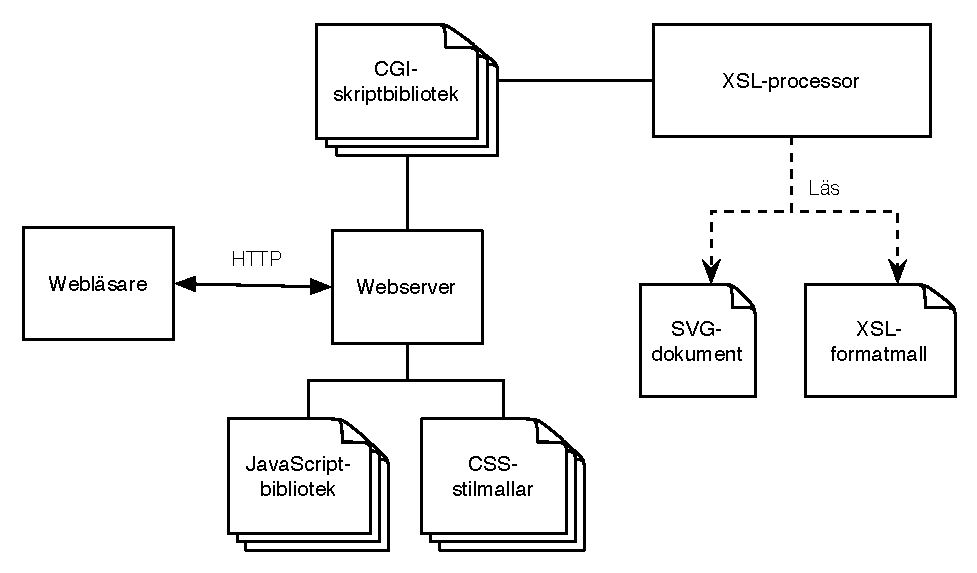
\includegraphics[width=\textwidth]{figurer/exekveringsvy.pdf}
\end{center}
\caption{Exekveringsvy}
\label{exekveringsvy}
 \end{figure}

\subsubsection{Webbl�sare}
Systemet st�djer endast webbl�saren Firefox version 3.5 eller senare.
Inga insticksprogram eller andra modifikationer kr�vs f�r att systemet ska
fungera som avsett.

\subsubsection{Webbserver}
Systemet anv�nder en standardinstallation av webbservern LightTPD.

\subsubsection{JavaScript-bibliotek}
Ett bibliotek med JavaScript-filer inneh�ller all funktionalitet som systemet
kr�ver p� klientsidan.
Det SVG-dokument som genererats av webservern inneh�ller referenser
till n�mnda JavaScript-filer som h�mtas automatiskt av webl�saren n�r dokumentet analyseras.

\subsubsection{CSS-stilmallar}
Det genererade SVG-dokumentets utseende styrs till viss
grad av stilmallar.

\subsubsection{CGI-skriptbibliotek}
Generering av berikade SVG-dokument och kopplingar till externa program sker via anrop 
till CGI-skript programmerade i Perl.

Varje externt program hanteras av ett specifikt CGI-skript.


\subsubsection{XSL-processor}
Ett CGI-skript berikar ett SVG-dokument vid f�rfr�gan. 
Detta inneb�r att det ursprungliga dokumentet l�mnas ober�rt och kan anv�ndas
i andra till�mpningar.

Systemet anv�nder XSL-processorn libxslt genom biblioteket
XML::LibXSLT.
% Systemets XSL-processor anv�nder det �ppna Perlbiblioteket XML::LibXSLT som
% fungerar som ett skal runt GNOME-projektets C-bibliotek libxslt.

\subsubsection{XSL-formatmall}
XSL-processorn anv�nder sig av denna formatmall f�r att transformera det
ursprungliga SVG-dokumentet och skapa bindningar mellan h�ndelser och
JavaScript-funktioner

Formatmallen inneh�ller �ven regler f�r att skapa referenser till
JavaScript-filer och CSS-stilmallar. %som klienten ska anv�nda sig av.

\subsubsection{SVG-dokument}
N�tverkskartor i SVG-format skapas av ett externt program med hj�lp av GraphViz.
% SVG-dokument som inneh�ller en grafisk representation av ett IP-n�tverk.
% Dessa dokument skapas av ett externt program med hj�lp av GraphViz.

%\section{Implementationsvy}
%Implementationsvyerna visar programkodsmodulernas viktigaste
%best�ndsdelar och hur dessa �r relaterade.
% Implementationsvyerna visar hur programkodsmodulerna �r relaterade och
% deras viktigaste delar i form av objekt, funktioner och konstanter.

\section{Implementationsvy �ver JavaScript-bibliotek}
JavaScript-biblioteket best�r av filer som hanterar systemets logik p� klientsidan.
Filerna visas i figur \vref{impl-js} och kommer att beskrivas i detalj nedan.

\begin{figure}[!hbtp]
\begin{center}
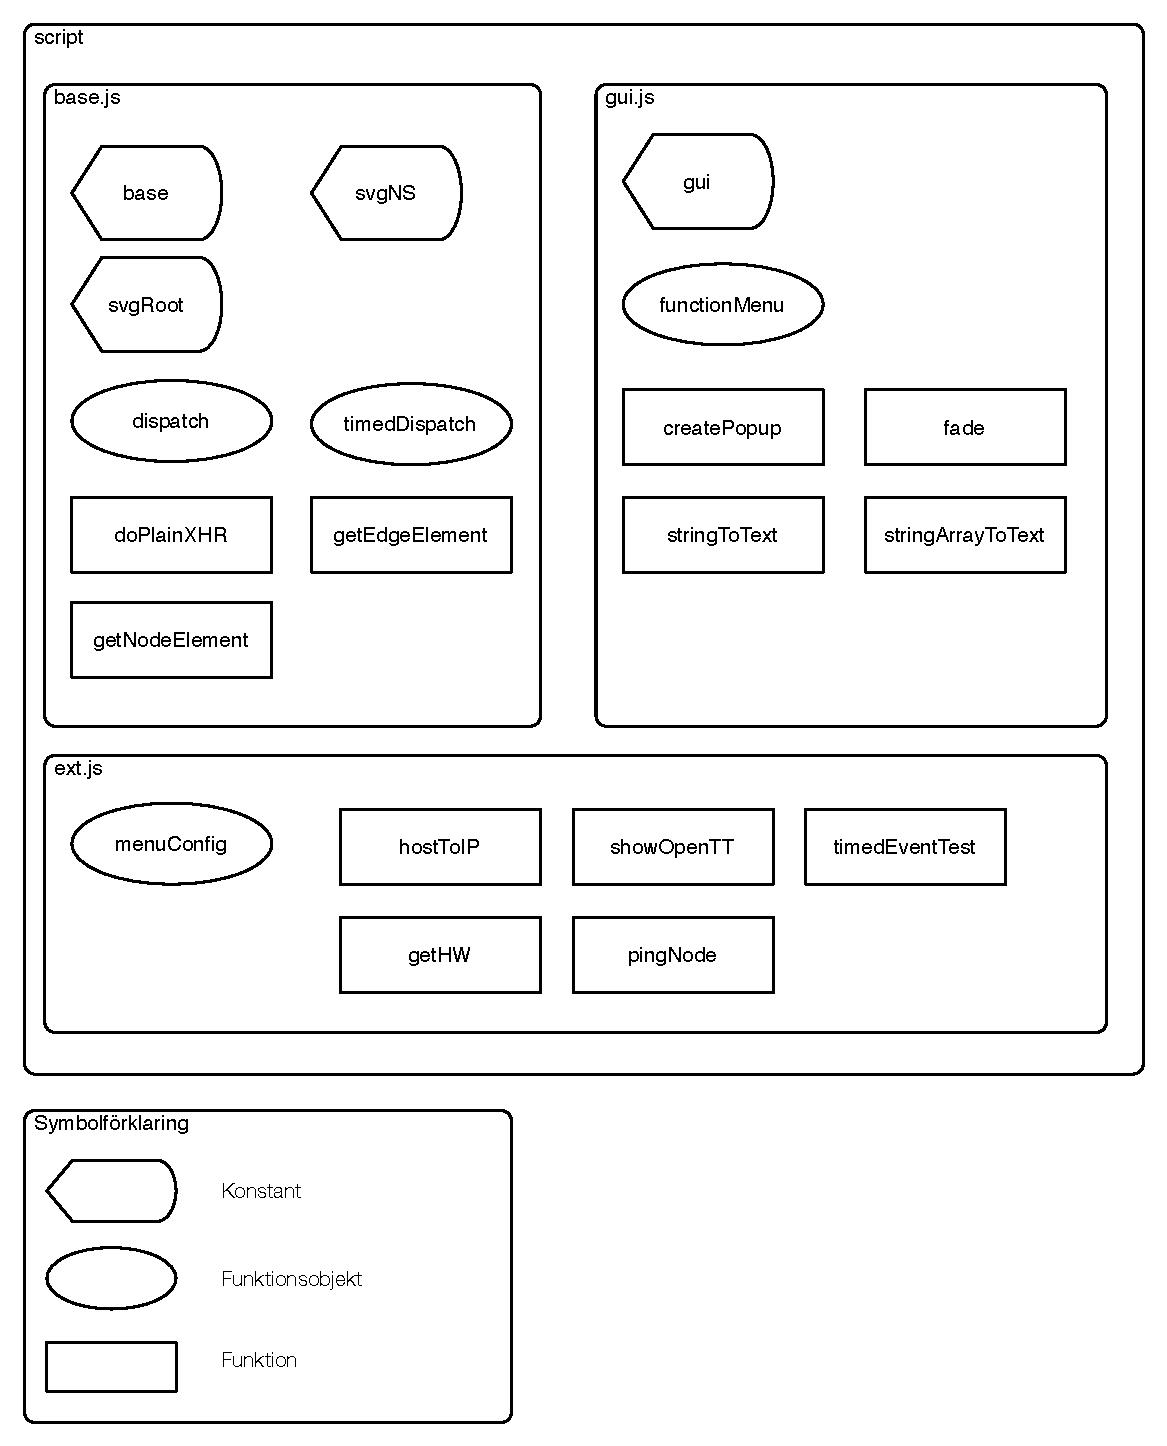
\includegraphics[width=\textwidth]{figurer/impl-js.pdf}
\end{center}
\caption{Implementationsvy �ver JavaScript-bibliotek}
\label{impl-js}
\end{figure}

\subsection{Base.js}
Filen \emph{base.js} inneh�ller de funktioner som �r bundna till h�ndelser i det
berikade SVG-dokumentet och hj�lpfunktioner som abstraherar delar av systemets
underliggande implementation.
B�de \emph{gui.js} och \emph{ext.js} kr�ver att denna fil �r exekverad innan de kan
analyseras av webl�saren.

\begin{itemize}
\item \emph{Base} �r ett namnrymdsobjekt som anv�nds f�r att skydda
 konstanter och funktioner fr�n namnkrockar d� variabler �r globala i
 JavaScript.
\item Konstanten \emph{svgRoot} h�ller en referens till SVG-dokumentets rot i DOM-tr�det.
\item \emph{SvgNS} inneh�ller XML-namnrymden f�r SVG och underl�ttar
  vid namnrymdsspecifika funktionsanrop i DOM.
 \item Funktionsobjektet \emph{dispatch} anv�nds f�r att hantera de
   funktionsanrop som bundits till h�ndelser i SVG-dokumentet och
   till�ter att flera funktioner utf�rs givet en specifik h�ndelse.
\item Funktionsobjektet \emph{timedDispatch} inneh�ller metoder f�r att
  l�gga till och ta bort funktioner som �r schemalagda att utf�ras i
  ett givet intervall.
\item Funktionen \emph{doPlainXHR} underl�ttar skapandet av asynkrona funktionsanrop
  till webservern.
\item \emph{GetEdgeElement} �r en av flera funktioner som abstraherar den
  underliggande representationen i systemet. Givet ett h�ndelseobjekt
  kan denna funktion ta fram det grafiska element som representerar en
  b�ge i grafen.
\item \emph{GetNodeElement} har samma funktionalitet som \emph{getEdgeElement}
  f�rutom att det element som representerar en nod i grafen returneras.
\end{itemize}

\subsection{Gui.js}
GUI st�r f�r graphic user interface vilket betyder grafiskt
anv�ndargr�nssnitt.
Denna JavaScript-fil inneh�ller funktioner kopplade till det grafiska gr�nssnittet.

\begin{itemize}
\item \emph{Gui} �r ett namnrymdsobjekt med samma funktion som \emph{base} i \emph{base.js}.
\item Funktionsobjektet \emph{functionMenu} inneh�ller metoder f�r att l�gga
  till verktygsprogram i en kontrollmeny som visas i SVG-dokumentet.
\item  Funktionen \emph{createPopup} skapar en dialogruta i SVG-dokumentet.
\item \emph{Fade} tonar ut eller in ett element i SVG-dokumentet
  och anv�nds av \emph{createPopup} och \emph{functionMenu}.
\item Funktionen \emph{stringToText} skapar en grupp inneh�llande ett
  textelement och kan anv�ndas f�r att l�gga till text i en dialogruta
  i SVG-dokumentet.
\item \emph{StringArrayToText} har samma funktionalitet som \emph{stringToText}
  f�rutom att den kan skapa flera textelement givet ett objekt med str�ngar.
\end{itemize}

\subsection{Ext.js}
Denna fil inneh�ller exempel p� hur systemet kan programmeras med
hj�lp av de ovan n�mnda filerna. 
Ut�kande av ny funktionalitet till systemet b�r g�ras i denna fil.

\begin{itemize}
\item \emph{MenuConfig} �r ett objekt inneh�llande en konfiguration som
  anv�nds vid skapandet av ett funktionsobjekt av typen \emph{functionMenu}.
\item Funktionen \emph{hostToIP} anropar ett CGI-skript p� webservern som returnerar
  ip-adressen som �r bunden till givet ett v�rdnamn.
\item Funktionen \emph{showOpenTT} demonstrerar hur ett
  verktygsprogram kan anropas utan hj�lp av \emph{doPlainXHR} och visa
  resultatet som ett HTML-dokument i ett nytt webl�sarf�nster. %utan att skapa en dialogruta med funktionen \emph{createPopup}.
\item \emph{TimedEventTest} �r ett exempel p� hur \emph{timedDispatch} kan
  utnyttjas f�r att en eller flera funktioner ska utf�ras regelbundet
  och automatiskt.
\item Funktionen \emph{getHW} anropar ett CGI-skript som returnerar information r�rande
  ett n�tverkselements h�rdvarubestyckning.
\item \emph{PingNode} s�nder en f�rfr�gan till ett CGI-skript att
  kontrollera om ett n�tverkselement �r �tkomlig via n�tverket
  webservern �r kopplad till.
\end{itemize}

\section{Implementationsvy �ver CGI-skriptbibliotek} %L�GG TILL INFO OM EXTERNT BIBLIOTEK
                                %OCH ATT DET INSTALLERAS MED CPAN
\label{sect:CGI-bibliotek}
De komponenter som ing�r i CGI-skriptbiblioteket och dess beroenden
visas i figur \vref{impl-cgi} och beskrivs nedan.
Samtliga CGI-skript �r utvecklade i programmeringsspr�ket Perl.
%De flesta CGI-skripten demonstrerar hur olika funktioner kan utf�ras
%p� webservern givet ett anrop fr�n en JavaScript-funktion p�
%klientsidan.

\begin{figure}[!hbtp]
\begin{center}
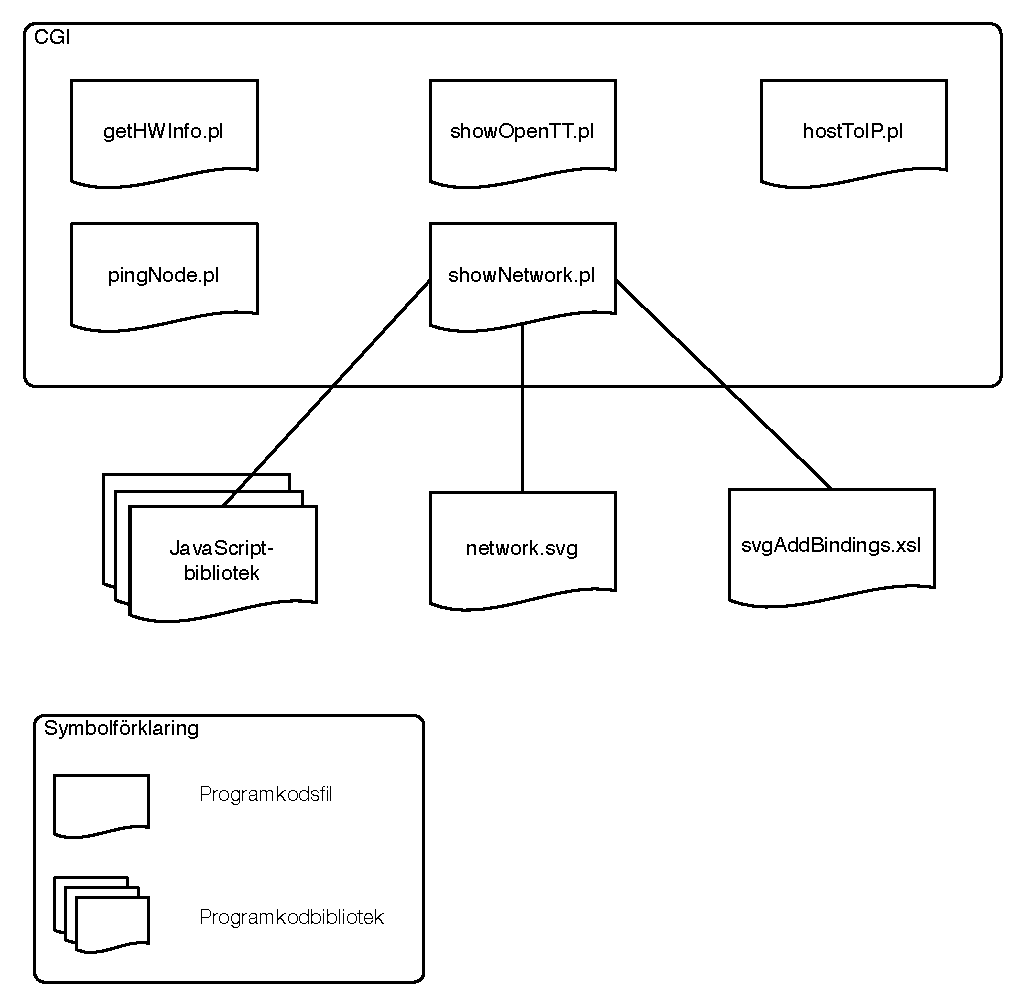
\includegraphics[width=\textwidth]{figurer/impl-cgi.pdf}
\end{center}
\caption{Implementationsvy �ver CGI-skriptbibliotek}
\label{impl-cgi}
\end{figure}


\subsection{GetHWInfo.pl}
CGI-skriptet \emph{getHWInfo.pl} h�mtar information r�rande ett n�tverkselements
h�rdvarubestyckning givet ett v�rdnamn.

\subsection{ShowOpenTT.pl}
Programmet \emph{showOpenTT.pl} skapar ett HTML-dokument och returnerar det till
klienten.

\subsection{HostToIP.pl}
Programmet \emph{hostToIP.pl} returnerar en IP-adress tillh�rande ett givet v�rdnamn.

\subsection{PingNode.pl}
CGI-skriptet \emph{pingNode.pl} kontrollerar om ett n�tverkselement kan n�s via det n�tverk
webservern �r ansluten till. 

\subsection{ShowNetwork.pl}
CGI-skriptet \emph{showNetwork.pl} utg�r den viktigaste delen av systemet d� det berikar
ett SVG-dokument med bindningar och referenser. 

Ett nytt dokument skapas baserat p� ett SVG-dokument som transformeras med
hj�lp av XSLT och returneras till webservern som d�refter skickar det
till klienten. 

XSL-transformationen kr�ver att ett externt Perlbibliotek anv�nds.
Biblioteket heter XML::LibXSLT och kan installeras genom CPAN.

\subsection{Network.svg}
Dokumentet \emph{network.svg} �r ett exempel p� en n�tverkskarta i SVG-format.
Det �r skapat av ett externt program med hj�lp av GraphViz.

\subsection{SvgAddBindings.xsl}
XSL-formatmallen inneh�ller regler f�r hur exempelfilen \emph{network.svg} ska
transformeras s� att det berikas med bindningar och referenser.

\section{Drifts�ttningsvy}

Drifts�ttningsvyn i figur \vref{driftvy} visar de h�rdvarukomponenter
som ing�r i systemet och var mjukvarukomponenterna �r utplacerade.

\begin{figure}[!hbtp] % Anv�nds float s� kan man ange H f�r exakt
                     % placering h�r
\begin{center}
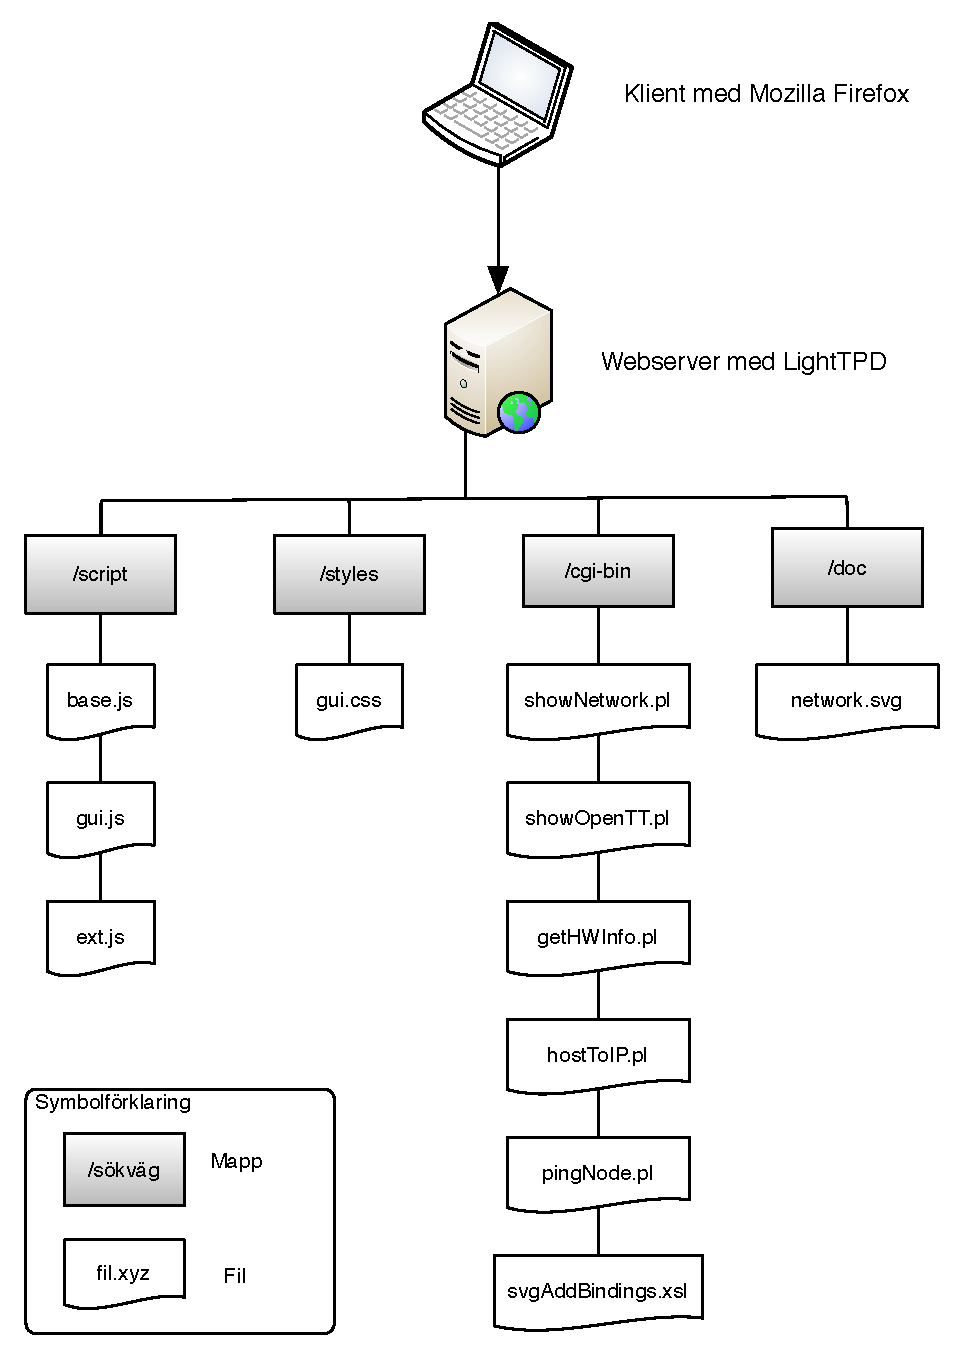
\includegraphics[width=\textwidth]{figurer/driftvy.pdf}
\end{center}
\caption{Drifts�ttningsvy}
\label{driftvy}
\end{figure}

\subsection{Klient}
Klienten best�r av en dator med ett operativsystem som �r kompatibelt med webbl�saren Firefox 3.5 eller
senare.

\subsection{Server}
Servern best�r av en dator med ett UNIX-baserat operativsystem med
webservern LightTDP installerad. 
I webserverns rotkatalog f�r webdokument finns det fyra mappar.

\begin{itemize}
\item \emph{/script} inneh�ller systemets JavaScript-filer.
\item \emph{/styles} inneh�ller CSS-stilmallar som styr dokumentens utseende.
\item \emph{/cgi-bin} inneh�ller alla CGI-skript som klienten kan anropa.
\item \emph{/doc} inneh�ller tillg�ngliga n�tverkskartor i form av
  SVG-dokument.
\end{itemize}




\section{Generering av SVG-dokument}
\label{sect:generering}
Klienten kan g�ra en f�rfr�gan till servern att leverera ett interaktivt SVG-dokument.
F�rfr�gan g�rs genom att ange en URL p� formen \\ 
\url{http://v�rdnamn.dom�n/cgi-bin/showNetwork.pl?network=namn.svg}.
Sekvensdiagrammet i figur \vref{fig:sekvens-svg} visar hur i detalj
hur genereringen g�r till.

\subsection{F�rfr�gan fr�n klient}
Generering av SVG-dokument sker genom att anropa ett CGI-skript p�
servern. Dokumentet returneras till klienten som beg�r att f� de filer
som �r refererade i det.

\begin{figure}[hbt]
\begin{center}
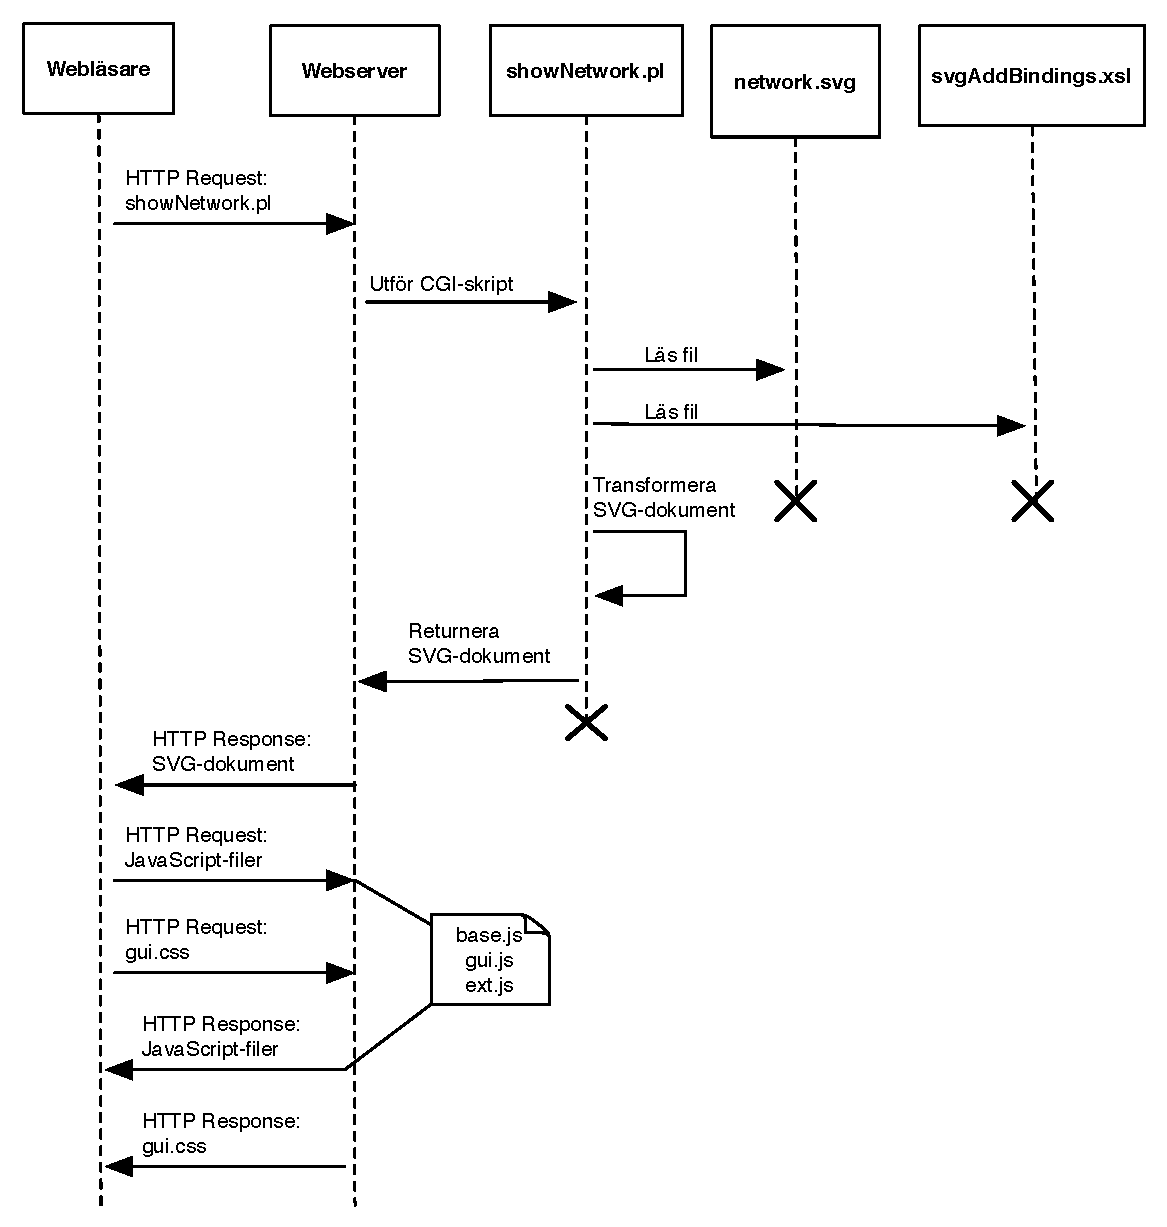
\includegraphics[width=\textwidth]{figurer/sekvensvy-showNetwork.pdf}
\end{center}
\caption{Sekvensdiagram �ver beg�ran av SVG-dokument}
\label{fig:sekvens-svg}
 \end{figure}

\subsection{Behandlande av f�rfr�gan}
CGI-skriptet \emph{showNetwork.pl} tar emot klientens f�rfr�gan om att
visa en n�tverkskarta och genererar ett nytt, berikat SVG-dokument. 
Den del i CGI-skriptet som utf�r transformationen och returnerar det
resulterande dokumentet visas i listning \vref{lst:cgi-trans}.

\lstset{language=Perl}
\begin{lstlisting}[float=htp, caption={XSL-transformation}, label=lst:cgi-trans]
  my $parser = XML::LibXML->new();
  my $xslt   = XML::LibXSLT->new();

  my $source    = $parser->parse_file( $svg_file );
  my $style_doc = $parser->parse_file( $xsl_file );

  my $stylesheet = $xslt->parse_stylesheet( $style_doc );

  my $result = $stylesheet->transform( $source );

  print $cgi->header( "image/svg+xml" );
  print $stylesheet->output_string( $result ); 

\end{lstlisting} %$

% Kommentarer till koden?


\section{XSL transformation}
\label{sect:xsl_trans}
CGI-skriptet showNetwork.pl tar emot en f�rfr�gan om att berika ett SVG-dokument. 
% Skriptet anv�nder sig av det �ppna Perlbiblioteket XML::LibXSLT och
% formatmallsfilen \emph{svgAddBindings.xsl}.
% Genom att skapa ett nytt dokument med bindningar och referenser till
% JavaScript l�mnas originaldokumenten or�rda. 
% F�rdelen med denna l�sning �r att de kan anv�ndas i andra till�mpningar som kan ha helt andra f�ruts�ttningar �n detta system.
%beh�ver man n�mna prestanda och nackdelar med att de genereras varje g�ng?

% Berikning av det efterfr�gade SVG-dokumentet sker med hj�lp av XSL
% transformation. F�r detta anv�nds det �ppna Perlbiblioteket
% \emph{XML::LibXSLT]. 

Formatmallsfilen \emph{svgAddBindings.xsl} inneh�ller regler f�r hur
dokumentet ska transformeras. 
De viktigaste transformationerna �r kopiering av element, referenser
till JavaScript-filer och bindningar mellan h�ndelser och funktioner.

\subsection{Identitetstransformation}
F�r att det nya berikade dokumentet ska inneh�lla all
information fr�n ursprungsdokumentet m�ste alla element och dess
attribut kopieras. 
Detta g�rs genom att applicera en s� kallad
identitetstransformation som visas i listning \vref{lst:xslt-ident}.

\begin{lstlisting}[float=htp, caption={Identitetstransformation}, label=lst:xslt-ident]
<xsl:template match="@*|node()">
  <xsl:copy>
    <xsl:apply-templates select="@*|node()"/>
  </xsl:copy>
</xsl:template>
\end{lstlisting}

\subsection{Till�gg av referenser till JavaScript-filer}
Roten i dokumentet �r ett SVG-element. En bindning till en
\emph{onload}-h�ndelse g�rs i elementets attributlista. Detta m�jligg�r
anrop till en JavaScript-funktion n�r dokumentet laddats f�rdigt.
Befintliga attribut kopieras.
Referenser till JavaScript-filer g�rs genom att skapa script-element
inneh�llande s�kv�gar till dessa. 
Notera att olika namnrymder m�ste anv�ndas d� olika typer av
XML-element anv�nds i formatmallen.
%\begin{lstlisting}[float=htp, caption={Till�gg av referenser till
%JavaScript}, label=xslt-jsref-kod]

Listning \vref{lst:xslt-ref} visar hur referenser l�ggs till.

\lstset{language=XSLT}
\begin{lstlisting}[float=htp, caption={Skapa referenser genom XSLT}, label=lst:xslt-ref]
<xsl:template match="/svg:svg">
  <xsl:copy>
    <xsl:copy-of select="@*" />
    <xsl:attribute name="onload">
        svg_onload(evt)
    </xsl:attribute> 
    <svg:script type="text/ecmascript" xlink:href="../script/base.js" />
    <svg:script type="text/ecmascript" xlink:href="../script/gui.js" />
    <svg:script type="text/ecmascript" xlink:href="../script/ext.js" />
    <xsl:apply-templates />
  </xsl:copy>
</xsl:template>
\end{lstlisting}

\subsection{Bindning av JavaScript-funktioner}
Det ursprungliga SVG-dokumentet inneh�ller tv� klasser av element som
�r intressanta f�r anv�ndaren att interagera med. Dessa �r klassen
\emph{nod} som representerar en nod i n�tverket som till
exempel en IP-router och klassen \emph{edge} som representerar en
f�rbindelse mellan tv� noder i n�tverket.
Bindningar ska skapas f�r dessa tv� klasser.
De h�ndelser som jag valt att skapa bindningar till �r \emph{onclick}, \emph{onmouseover} och
\emph{onmouseout} vilka �r en delm�ngd av de befintliga
mus-h�ndelserna i DOM level 2. %ref till svg 10 ref, Kursivera DOM?
Listning \vref{lst:xslt-jsbind} visar hur bindningen genomf�rs.

\begin{lstlisting}[float=htp, caption={Bindning av JavaScript-funktioner}, label=lst:xslt-jsbind]
<xsl:template match="svg:g">
  <xsl:copy>
    <xsl:if test="@class='node'">
      <xsl:attribute name="onclick">
          node_onclick(evt)
      </xsl:attribute>
      <xsl:attribute name="onmouseover">
          node_onmouseover(evt)
      </xsl:attribute>
      <xsl:attribute name="onmouseout">
          node_onmouseout(evt)
      </xsl:attribute>
    </xsl:if>
    <xsl:if test="@class='edge'">
      <xsl:attribute name="onclick">
          edge_onclick(evt)
      </xsl:attribute>
      <xsl:attribute name="onmouseover">
          edge_onmouseover(evt)
      </xsl:attribute>
      <xsl:attribute name="onmouseout">
          edge_onmouseout(evt)
      </xsl:attribute>
    </xsl:if>
    <xsl:apply-templates select="@*|node()" />
  </xsl:copy>
</xsl:template>
\end{lstlisting}

\section{Asynkrona anrop via XMLHttpRequest}
\label{sect:xhr}
Klientens anrop till servern att utf�ra program ska enligt kravspecifikationen g�ras asynkront. 
Detta inneb�r att klientens gr�nssnitt som utg�rs av SVG-dokumentet ej l�ses medan den v�ntar p� svar fr�n servern. 

F�r att underl�tta asynkrona anrop har en hj�lpfunktion skapats kallad \emph{doPlainXHR}.
Funktionen anv�nder parametrar som anger p� vilket s�tt anropet ska ske (Get eller Post), vilken URL den ska utf�ra anropet mot och en funktion som ska utf�ras n�r servern skickar ett svar. 
\emph{doPlainXHR} returnerar serverns svar som ren text men objektet XMLHttpRequest kan �ven returnera svaret som XML.

Ett XMLHttpRequest-objekt kan endast hantera ett anrop i taget. 
Ett svar fr�n ett anrop m�ste ges innan objektet kan utf�ra n�sta anrop.
Eftersom \emph{doPlainXHR} i listning \vref{lst:xhr} skapar ett nytt XMLHttpRequest-objekt vid varje anrop d�ljs denna begr�nsning f�r anv�ndaren.

\lstset{language=Java}
\begin{lstlisting}[float=htp, caption={XMLHttpRequest}, label=lst:xhr]
base.doPlainXHR = function( method, url, fun ) {
    var xhr = new XMLHttpRequest();
    xhr.open( method, url );
    xhr.onreadystatechange = function() {

        // Request is done
        if (xhr.readyState == 4) {

            // Check status code and handle errors
            if ( xhr.status == 200 ) {    // it went well
                fun( xhr.responseText );  
            } else if ( xhr.status == 404 ) {
                base.showNotFoundError( url );
            } else if ( xhr.status == 500 ) {
                base.showInternalError( url );
            } else {
                base.showUnknownError( xhr.responseText );
            }
            
        }
    };
    xhr.send( null );
}
\end{lstlisting}


\section{Expedieringsobjekt}
\label{sect:expedieringsobjekt}
Systemet har st�d f�r att utf�ra flera funktioner givet en h�ndelse i SVG-dokumentet. 
Detta �r implementerat genom expedieringsobjekt som inneh�ller en datastruktur med nyckel/v�rde-par f�r ett godtyckligt antal funktioner.
N�r JavaScript-filen \emph{base.js} laddas av webl�saren skapas ett expedieringsobjekt f�r varje definierad h�ndelse i SVG-dokumentet.

\subsection{Funktion f�r att skapa expedieringsobjekt}
Funktionen \emph{makeDispatch} i listning \vref{lst:js-exp} skapar ett nytt expedieringsobjekt och returnerar ett gr�nssnitt till dess metoder.
Metoderna g�r det m�jligt att l�gga till, ta bort och lista funktioner i objektet.
Metoden \emph{handleEvent} tar ett h�ndelseobjekt som parameter och utf�r alla funktioner som f�r tillf�llet finns i expedieringsobjektets datastruktur.


\begin{lstlisting}[float=htp, caption={Skapa expedieringsobjekt}, label=lst:js-exp]
base.makeDispatch = function() { 
    
    var funMap = {}; // functions

    // Return the interface to the dispatch object
   return { 
       addFunction: function( name, fun ) { 
           funMap[name] = fun;
       },
       
       removeFunction: function( name ) {
           delete funMap[name];
       },
       
       listFunctions: function() {
           var names = [];
           for (name in funMap) {
               // hasOwnProperty is used so that things from the prototype chain
               // isn't dragged up here
               if (funMap.hasOwnProperty( name )) {
                   names.push( name );
               }
           }
           return names;
       },

        handleEvent: function( evt ) {
            for (name in funMap) {
                if (funMap.hasOwnProperty( name )) {
                    funMap[name]( evt );
                }
            }
        }

   }; // end return
}

\end{lstlisting}



\subsection{Till�gg av funktioner till expedieringsobjekten}
Kodexemplet i listning \vref{lst:exp-addfun} visar hur en funktion kan l�ggas till ett expedieringsobjekt f�r h�ndelsen \emph{onclick}.
N�r h�ndelsen avfyras kommer ett asynkront anrop att genomf�ras till ett CGI-skript med namnet \emph{ajaxTest.pl}.
Resultatet av k�rningen av skriptet kommer att visas i en dialogruta i webl�saren.

\begin{lstlisting}[float=htp, caption={Till�gg av funktioner i expedieringsobjekt}, label=lst:exp-addfun]
base.edgeClickDispatch.addFunction( 'ajax', function( evt )
{
    base.makePlainXMLRequest( 'GET', '/cgi-bin/ajaxTest.pl?key=edge_ajax',
    function( response ) 
    {
      alert( response ) 
    } );
} );
\end{lstlisting}


\section{Funktionsmeny}
N�r en anv�ndare klickar p� en nod i SVG-dokumentet visas en meny som listar de funktioner som finns tillg�ngliga. 
N�r dessa funktioner utf�rs kan de anv�nda den aktuella noden som parameter.

Funktionsmenyn �r kopplad till ett funktionsobjekt som skapas n�r dokumentet laddats klart av webl�saren.
Listning \vref{lst:createMenu} visar hur objektet kan skapas.

\begin{lstlisting}[float=htp, caption={Skapa funktionsmeny}, label=lst:createMenu]
base.svgLoadDispatch.addFunction( 'create_menu', 
                                  function() { 
                                      gui.functionMenu.create( menuConfig ) } );

\end{lstlisting}



\subsection{Konfiguration av funktionsmeny}
N�r funktionsmenyn skapas kan ett konfigurationsobjekt anges som parameter.
Detta objekt inneh�ller information om vilka dimensioner menyn ska ha, hur den ska se ut och vilka funktioner den ska inneh�lla. 
Funktionerna anges som ett nyckel/v�rde-par d�r v�rdet �r en referens
till en namngiven eller anonym funktion.
Om v�rden saknas i konfigurationsobjektet eller om objektet saknas helt s� skapas funktionsmenyn med f�rvalda v�rden f�r dessa.
Listning \vref{lst:menuConf} visar ett exempel p� ett konfigurationsobjekt.

\begin{lstlisting}[float=htp, caption={Konfigurationsobjekt f�r meny}, label=lst:menuConf]
var menuConfig = { 
  x: base.viewBoxCenter - 400, y: 0,
  width: 800, height: 200, 
  rx: 5, ry: 5,
  functions: { 'Get IP adress': hostToIP,
    'Show open trouble tickets': showOpenTT,
    'Toggle timed events': timedEventTest,
    'Ping node': pingNode,
    'Show hardware info': getHW
  } 
};
\end{lstlisting}



\subsection{Funktionmenysobjektets gr�nssnitt}
N�r funktionmenyn skapas och initieras med en konfiguration returneras funktionsmenyobjektets gr�nssnitt.
Gr�nssnittet inneh�ller metoder f�r att visa och g�mma menyn, l�gga till och ta bort funktioner ur menyn.
Det g�r �ven att erh�lla en referens till det element anv�ndaren senast klickade p� och var orsaken till att menyn visades.
Listning \vref{lst:menuInterface} visar gr�nssnittet som returneras n�r funktionsmenyobjektet skapas.

\begin{lstlisting}[float=htp, caption={Funktionsmenyns gr�nssnitt}, label=lst:menuInterface]
 return {
         show: function( evt ) {
                menu.setAttribute( 'display', 'block' );
                gui.fadeIn( menu );
                if (evt) currentElement = evt.target;
        },
        
        hide: function( evt ) {
            gui.fadeOut( menu, function() { 
                menu.setAttribute( 'display', 'none'); } );
            if (evt) currentElement = evt.target;
        },
        
         addFunctions: function( functions ) {
             this.removeFunctions();
             this.createFunctionGroup( functions, menuGroup );
        },
         
         removeFunctions: function() {
             menuGroup.removeChild( 'functionGroup' );
         },
         
        currentElement: function() { return currentElement; },
}
\end{lstlisting}


% Diskussion f�r hela implementationskapitlet
\section{Sammanfattning}
I detta kapitel har jag redovisat implementationen av ett system f�r interaktiv
visualisering av IP-n�tverk. Implementationen bygger p�
kravspecifikationen i kapitel \vref{chap:krav} och resultatet av min
problemanalys i kapitel \vref{chap:analys}.
Kapitlet b�rjade med att ge en �versikt �ver systemet f�r att
sedan i djupare detalj visa varje komponent. 
Av praktiska och utrymmessk�l har jag valt att enbart visa programkod f�r de viktigaste
delarna av systemet.

I n�sta kapitel utv�rderar jag resultatet av implementationen och
visar testningen av kraven i kravspecifikationen.


\chapter{Testning och utv�rdering}
\label{chap:test_och_utv}
F�r att kunna avg�ra om ett utvecklingsprojekt n�tt en punkt d�r det
kan anses vara f�rdigt m�ste tester genomf�ras f�r att verifiera
kravspecifikationen.
Jag anv�nde tester f�r att avg�ra n�r varje del av
systemet var f�rdigst�llt och d�rf�r var jag tvungen att i samband med
framst�llandet av kravspecifikationen ocks� definiera hur kraven i
denna skulle testas. En lista med testerna redovisades i kapitel \vref{sect:test_av_krav}.
F�r att testerna ska kunna genomf�ras m�ste en representativ testmilj�
s�ttas upp. En detaljerad beskrivning av testmilj�n ges i avsnittet som
behandlar testningen av kravspecifikationen.

Kapitlet inleds med att visa hur syftet med arbetet uppfyllts
f�ljt av en utv�rdering av de designval jag gjort i implementationen
av systemet.
Avslutningsvis redovisar min testning av kravspecifikationen och
sammanfattar hur v�l systemet uppfyller kraven.


\section{Uppfyllande av syfte}
Syftet med detta arbete som jag skrev i inledningen var att utveckla ett prototypsystem som g�r n�tverkskartor interaktiva.
Det skulle vara m�jligt att anropa befintliga verktygsprogram via dessa kartor.
I kapitel \vref{chap:implementation} beskrev jag ett system som
uppfyller f�ljande:

\begin{itemize}
\item Genererar interaktiva n�tverkskartor baserade p� SVG-dokument
  och JavaScript.
\item Till�ter anrop av CGI-skript p� en webbserver genom att en
  anv�ndare interagerar med n�tverkskartan.
\item Visar resultat fr�n k�rning av CGI-skript p� webbservern i
  n�tverkskartan.
\end{itemize}

De tre punkterna ovan anser jag tillsammans uppfyller syftet med detta
arbete.

% \section{Inkludera SVG i XHTML}
% Det �r m�jligt att inkludera SVG-dokumentet som representerar ett IP-n�tverk i ett XHTML-dokument.
% P� detta s�tt kan befintliga XHTML-baserade webapplikationer ut�kas med den funktionalitet
% som erbjuds av detta system. 


\section{Utv�rdering av designval}
I kapitel \vref{chap:analys} beskrev jag de designval jag
funnit f�r att l�sa var och ett av de fyra delproblem jag brutit ned
arbetet till.
I detta avsnitt, som har samma uppdelning som kapitel
\vref{chap:analys}, utv�rderar jag de alternativ jag valde i
implementationen av systemet.
% \begin{itemize}
% \item Bindning av JavaScript-funktioner.
% \item Hantering av anv�ndarinitierade h�ndelser.
% \item Anrop fr�n klient till server.
% \item Behandling av anrop fr�n klient.
% \end{itemize}

\subsection{Bindning av JavaScript-funktioner}
%val
I kapitel \vref{sect:xsl_trans} framg�r det att jag valt alternativet
att skapa ett tempor�rt SVG-dokument berikat med bindningar genom att
transformera originaldokumentet genom XSLT p� serversidan.

%motivering
Alternativet att anv�nda XSLT valdes f�r att originaldokumentet ska l�mnas ober�rt. 
Detta inneb�r att originaldokumentet kan anv�ndas i andra till�mpningar som inte beh�ver vara beroende
av hur detta system anv�nder det.
�ndringar i systemet kan d�rf�r g�ras utan att andra till�mpningar ber�rs.

% Flyttas till Framtida arbete:
% F�r att minimera denna upprepade generering skulle ett nyligen genererat dokument kunna sparas
% i ett ``cacheminne'' under en begr�nsad tid. Tyv�rr medf�r detta fler
% skrivningar till och l�sningar fr�n h�rddisk.

%utv�rdering
En nackdel med den valda l�sningen �r att ett nytt SVG-dokument m�ste genereras varje g�ng en klient
beg�r att f� dokumentet f�r en specifik del av n�tverket. 
Systemet har ej testats under last med m�nga klienter som beg�r
n�tverkskartor.
Under arbetet uppfattade jag genereringen av dokumenten som mycket snabb.


\subsection{Hantering av anv�ndarinitierade h�ndelser}
%val
N�r ett SVG-dokument transformeras med XSLT skapas nya attribut i utvalda elements attributlistor.
Dessa attribut binder en h�ndelse till en JavaScript-funktion.
Systemet anv�nder sig av flera expedieringsobjekt, ett per h�ndelse
och element. I kapitel \vref{sect:expedieringsobjekt} visade jag
implementationen av de expedieringsobjekt som anv�nds i systemet.

%motivering
Dessa expedieringsobjekt kan h�lla ett godtyckligt antal (inklusive noll) funktioner som ska utf�ras n�r
en h�ndelse avfyras.
Detta inneb�r att systemet enkelt kan byggas ut genom att l�gga till, ta bort och f�r�ndra de funktioner
som expedieringsobjekten h�ller.
Alternativet till att anv�nda expedieringsobjekt f�r att ta hand om
utl�sta h�ndelser �r som jag skrev i kapitel \vref{sect:h�ndelser} att
programmera en specialiserad funktion f�r varje element och
h�ndelse. Jag anser att det senare alternativet g�r systemet sv�rare att ut�ka
med ny funktionalitet. Ut�kningar kr�ver �ven �ndringar i
funktionernas programkod vilket kan leda till att nya
defekter introduceras i funktionernas programkod.

%utv�rdering
De flesta h�ndelser i systemet kr�ver dock enbart att en funktion utf�rs och expedieringsobjekten medf�r 
d�rf�r on�diga ber�kningar i dessa fall. Expedieringsobjekten �r enkla att ut�ka med nya funktioner under
exekvering och jag anser att det �r en stor f�rdel att hantera alla
typer av h�ndelser p� samma s�tt.

\subsection{Anrop fr�n klient till server}
%val
I kapitel \vref{sect:anrop} visade jag tv� alternativ f�r hur
asynkrona anrop fr�n klient till server kan ske. Jag valde att anv�nda
det f�rsta alternativet med XML\-Http\-Request-objektet .

%motivering
XMLHttpRequest fungerar som vilket JavaScript-objekt som helst. Jag
anser att XMLHttpRequest-objektet som visades i listning
\vref{lst:xhr} �r enkelt att anv�nda.
Alternativet att anv�nda ett script-element f�r asynkron kommunikation �r inte aktuellt d� det inte finns n�got
behov att anropa servrar med olika v�rdnamn. 
Begr�nsningen i vilka v�rdnamn som f�r anv�ndas vid serveranrop finns inte l�ngre kvar i
Firefox 3.5 och senare.

%utv�rdering
%Enligt kravspecifikationen f�r anrop till servern endast ske
%asynkront. XML\-Http\-Request-objektet uppfyller detta krav.
Ett problem med att anv�nda asynkron kommunikation enligt den valda
l�sningen �r att anv�ndaren ej kan se om klienten anropar servern via webbl�sarens gr�nssnitt.


\subsection{Behandling av anrop fr�n klient}
%val
I kapitel \vref{sect:CGI-bibliotek} visade jag att systemet har ett specifikt CGI-skript f�r varje funktion som anv�ndaren kan anropa fr�n funktionsmenyn i anv�ndargr�nssnittet.
CGI-skripten ansvarar f�r att ta emot och analysera anropet, utf�ra funktionen och returnera resultatet till klienten.
% D� l�sningen att anv�nda XMLHttpRequest-objektet valdes finns det tv� olika s�tt att leverera 
% resultatet till klienten.
% Resultaten kan antingen levereras som ett XML-objekt eller som ren text.
% Systemet anv�nder det senare alternativet d� funktionerna p� klientsidan ej beh�ver g�ra n�gon
% avancerad analys eller tolkning av resultatet. 

%motivering
N�r systemet ut�kas med nya funktioner beh�ver inga till�gg eller �ndringar g�ras i de befintliga
programmen p� servern. 
Det minskar risken att inf�ra defekter i den befintliga programkoden.

%utv�rdering
En nackdel �r att duplicering av programkod kan ske d� flera CGI-skript 
hanterar klientens anrop p� samma eller liknande s�tt.
Det kan vara sv�rt att �verblicka systemet om det ut�kas med 
m�nga CGI-skript. 
Det finns inga krav p� hur GCI-skriptens gr�nssnitt ska se ut vilket
kan medf�ra en risk att deras utformning skiljer sig helt mellan
skripten.
Detta i sin tur kan g�ra det sv�rare att underh�lla systemet.


\section{Uppfyllande av kravspecifikation}
I detta avsnitt redovisar jag hur jag testat systemet mot
kravspecifikationen och huruvida kraven blivit uppfyllda.
Jag har p� klientsidan anv�nt f�ljande testmilj�:
\begin{itemize}
\item Webbl�saren Firefox version 3.5 och 3.6.
\item Microsoft Windows XP med Service Pack 3.
\item Apple MacOSX version 10.6.3.
\end{itemize}


P� serversidan har jag anv�nt f�ljande testmilj�:
\begin{itemize}
\item Debian 5.0.4 f�r 64-bitars arkitektur.
\item Webbservern LightTPD 1.4.26.
\end{itemize}

\subsection{Obligatoriska krav}
  
\subsubsection*{K1 -- Mjukvarupaketet GraphViz ska anv�ndas f�r att generera SVG-dokument}
De SVG-dokument systemet hanterar �r skapade av ett externt program som anv�nder
GraphViz.

\subsubsection*{K2 -- Den grafiska representationen ska vara i formatet SVG}
Anv�ndargr�nssnittet p� klienten utg�rs av ett SVG-dokument.

\subsubsection*{K3 -- Applikationer p� serversidan ska vara av typen CGI-skript skrivna i 
  programmeringsspr�ket Perl}
Alla applikationer p� serversidan �r skrivna i Perl och anv�nder CGI.

\subsubsection*{K4 -- Applikationer p� klientsidan ska vara skrivna i
  programmeringsspr�ket JavaScript}
All programkod i systemet som utf�rs p� klienten �r skriven i JavaScript.

\subsubsection*{K5 -- Webbservern som anv�nds i systemet ska vara LightTPD}
Systemet �r utvecklat f�r och testat p� webbservern LightTPD.

\subsubsection*{K6 -- Systemet ska st�dja webbl�saren Firefox version 3.5 eller senare}
Systemet �r utvecklat f�r Firefox version 3.6.
Jag utf�rde de tillg�ngliga funktionerna i klientsidans gr�nssnitt i Firefox version 3.5 och version 3.6.
Systemets funktionalitet skiljde sig inte mellan de tv�
webbl�sarversionerna och SVG-dokumentet renderades korrekt i b�gge.

\subsubsection*{K7 -- Ett befintligt verktygsprogram ska kunna anropas via anv�ndarinteraktion
  med SVG-dokument i webbl�saren}
Detta krav �r ej uppfyllt p� grund av omst�ndigheter som gjorde det
om�jligt att testa systemet i uppdragsgivarens n�tverk inom arbetets tidsram.
Det g�r dock att exekvera ett godtyckligt program p� serversidan genom
att anv�nda CGI. Programmet kan vara ett verktygsprogram.
%Jag har i kapitel \vref{sect:CGI-bibliotek} visat att systemet p� serversidan kan utf�ra godtyckliga program.
Uppdragsgivaren har godtagit detta.

\subsubsection*{K8 -- Anrop enligt krav K7 ska ske asynkront}
Alla anrop till servern sker genom att anv�nda funktionen \emph{doPlainXHR}.
Funktionen anv�nder XMLHttpRequest-objektets metod \emph{open} med 
det f�rvalda v�rdet att operationen ska utf�ras asynkront.
F�r att testa detta krav f�rs�krade jag mig f�rst om att all
programkod som genomf�r anrop till servern anv�nder \emph{doPlainXHR}.
Efter det programmerade jag testprogram p� serversidan som tog emot
anropet, genomf�rde en paus under tre sekunder och returnerade en
textstr�ng till klienten.
Under tiden som testprogrammet exekverades p� servern verifierade jag
att det gick att interagera med n�tverkskartan och utf�ra funktionerna i funktionsmenyn.

\subsubsection*{K9 -- Resultatet av k�rningen av verktygsprogrammet ska visas i
  den webbl�sare d�r anropet initierades}
CGI-skripten p� serversidan returnerar resultaten av k�rningen av
verktygsprogram till den anropande klienten. Enligt
RFC\footnote{Request for comments. Ett dokument som beskriver ett
  f�rslag till standard.}
3875\cite{rfc:cgi} som beskriver CGI, ska en webbserver omvandla ett
svar fr�n ett CGI-skript till ett svar till den anropande klienten.
Jag genomf�rde testade detta genom att utf�ra funktionerna i
funktionsmenyn och notera om ett svar returnerades till webbl�saren
och visades i SVG-dokumentet.
Precis som f�r krav K7 har detta krav ej testats med befintliga verktygsprogram men
principen �r densamma oavsett vilket program som utf�rs p� serversidan.

\subsubsection*{K10 -- Interaktion med SVG-dokument p� klientsidan ska ej p�verka 
  originaldokumentet p� serversidan}
N�r en klient beg�r att f� ett berikat SVG-dokument fr�n webbservern genereras en tempor�r 
kopia av originaldokumentet.
Interaktioner med dokumentet p� klientsidan kan s�ledes ej p�verka
originaldokumentet.
Jag testade detta krav genom att utf�ra de tillg�ngliga funktionerna p�
klientsidan och kontrollerade att originaldokumentet p� servern var of�r�ndrat.

\subsubsection*{K11 -- Alla komponenter i systemet ska anv�nda �ppen
  mjukvara}
De komponenter som ing�r i systemet �r alla av typen �ppen mjukvara.
Komponenterna �r:
\begin{itemize}
\item Webbl�saren Firefox.
\item Webbservern LightTPD med den inkluderade
implementationen av CGI.
\item Biblioteket XML::LibXSLT som inkluderar biblioteket libxslt.
\item Mjukvarupaketet GraphViz.
\end{itemize}
% �r det alla komponenter kravet h�nvisar till? JA!(?) :-)

\subsection{Frivilliga krav}

\begin{figure}[!hbt]
\begin{center}
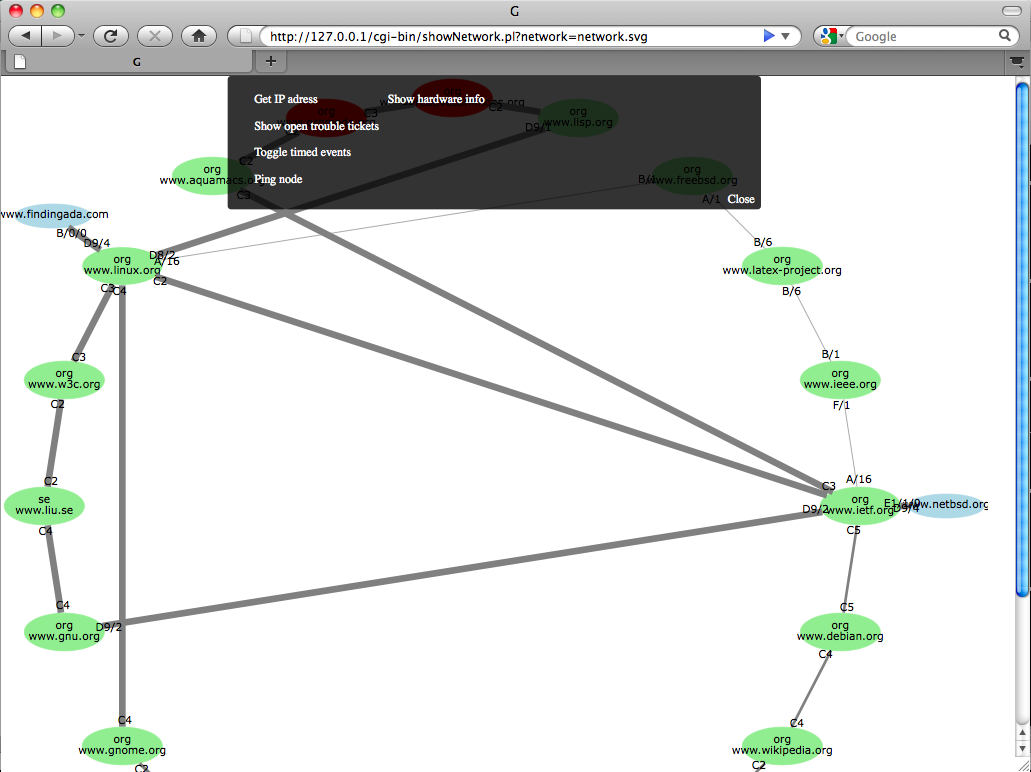
\includegraphics[width=\textwidth]{figurer/funktionsmeny.png}
\end{center}
\caption{Sk�rmavbild som visar funktionsmenyn}
\label{pic:funktionsmeny}
\end{figure}

\subsubsection*{F1 -- N�r en anv�ndare h�gerklickar p� ett element i SVG-dokumentet ska en lista
  med tillg�ngliga funktioner visas}
Kravet �r ej uppfyllt men en liknande funktion implementerades.
N�r en anv�ndare klickar p� en nod i grafen visas en meny med funktioner (funktionsmenyn) i mitten av dokumentets �vre del.
Figur \vref{pic:funktionsmeny} visar funktionsmenyn i anv�ndargr�nssnittet.

Att visa en meny p� den position i dokumentet d�r anv�ndaren h�gerklickar �r problematiskt.

Problemet grundas i hur x- och y-koordinater anv�nds i webbl�saren och dokumentet.
N�r ett nytt element ska l�ggas till anges dess x- och y-koordinater relativt dokumentets �vre v�nstra h�rn.
N�r en h�ndelse avfyras i webbl�saren inneh�ller h�ndelseobjektet x- och y-koordinater som �r relativa med
webbl�sarf�nstrets �vre v�nstra h�rn. 
Om dokumentet f�rstoras s� att det inte ryms i webbl�sarf�nstret kan det flyttas med hj�lp av rullningslister
i webbl�saren. 
Sker detta g�r det inte att anv�nda de koordinater som h�ndelseobjektet inneh�ller f�r att skapa ett nytt
element p� platsen anv�ndaren klickade. 
H�ndelseobjektets koordinater och dokumentets koordinater tillh�r olika koordinatsystem.
Koordinaternas v�rden anger pixlar p� sk�rmen.

Firefox tillhandah�ller v�rden f�r hur m�nga pixlar ett dokument flyttats med rullningslisterna.
Jag antog att det med dessa v�rden gick att �vers�tta de koordinater som h�ndelseobjektet
inneh�ll till samma koordinatsystem som dokumentet anv�nde. 

Jag tog fram denna formel d�r $d$ st�r f�r dokument, $h$ f�r h�ndelse och $f$ f�r f�rflyttning:
\[ (x,y)_{d}=(x_{h}+x_{f}, y_{h}+y_{f}) \]

Dessv�rre �r ekvationen ej var sann f�r varje v�rde $f$.
Ju mer dokumentet flyttas i webbl�saren desto st�rre blir felet.
Detta inneb�r att menyn visas l�ngre fr�n muspekaren ju mer dokumentet flyttas i webbl�sarf�nstret.


\subsubsection*{F2 -- Listan i krav F1 ska genereras baserat p� elementets identifierare}
Detta krav har ej uppfyllts d� jag anser att det tar f�r l�ng tid att utveckla ett system f�r att knyta en viss typ
av h�rdvara till en given m�ngd funktioner.

\subsubsection*{F3 -- Systemet ska inneh�lla funktionalitet f�r att automatiskt anropa ett
  verktygsprogram baserat p� en timer}
Detta krav har ej uppfyllts d� det inte har getts m�jlighet att anropa verktygsprogram fr�n webbservern.
Jag har utvecklat en timer som kan anropa ett godtyckligt antal JavaScript-funktioner p� klientsidan.
En anropad funktion kan i sin tur anropa ett program p� serversidan.

\section{Sammanfattning}
Systemet som beskrevs i kapitel \vref{chap:implementation} uppfyllde
de obligatoriska kraven K1 till och med K12 med undantag f�r krav K7.
Detta krav �r ej uppfyllt p� grund av omst�ndigheter som gjorde det
om�jligt att testa systemet i uppdragsgivarens n�tverk inom arbetets
tidsram.
CGI-skript p� webbservern kan dock exekvera ett godtyckligt program p�
serversidan vilket inneb�r att det inte finns n�gra tekniska
begr�nsningar i att koppla ihop verktygsprogrammen med systemet.

Inget av de frivilliga kraven uppfylldes enligt
kravspecifikationen. Ist�llet f�r att visa en meny med funktioner f�r
anv�ndaren n�r denne h�gerklickar p� ett element i n�tverkskartan
enligt krav F1,  visas menyn h�gst upp i mitten av
n�tverkskartan.
G�llande krav F3 s� implementerade jag en timerfunktion enligt
kravspecifikationen. 
Jag implementerade en timerfunktion enligt krav F3 men kunde tyv�rr inte uppfylla kravet helt d� jag
ej kopplade ihop timern med befintliga verktygsprogram.

\chapter{Diskussion och slutsatser}
I detta kapitel sammanfattar jag det arbete som beskrivits rapporten.
Jag inleder kapitlet med en diskussion r�rande systemet. D�refter
kommenterar jag valet av metod f�r arbetet f�ljt av en diskussion om
hur systemet skulle kunna vidareutvecklas. Avslutningsvis n�mner jag
n�gra av de erfarenheter jag f�tt under arbetet.


\section{Diskussion}
% m�l med arbetet
Mitt m�l med detta arbete var att ett system
f�r att m�jligg�ra interaktiv visualisering av IP-n�tverk och koppla
ihop noder i n�tverket med befintliga verktygsprogram. 
Arbetet resulterade i:
\begin{itemize}
\item Ett XSL-program som berikar ett befintligt SVG-dokument skapat
  genom GraphViz med bindningar till JavaScript-funktioner.
\item Tre JavaScript-bibliotek med funktioner som g�r n�tverkskartan interaktiv och
  kopplar ihop denna med CGI-skript p� webbservern.
\item CGI-skript f�r att hantera anrop fr�n webbl�saren och utf�ra
  �nskade funktioner.
\item En CSS-stilmall som styr utseendet av n�tverkskartan.
\end{itemize}

Som jag n�mnde i kapitel \vref{chap:test_och_utv}, uppfyllde systemet
alla obligatoriska krav i kravspecifikationen f�rutom kravet att
befintliga verktygsprogram ska kunna anropas. Det finns inga tekniska
begr�nsningar i systemet som om�jligg�r anrop av
verktygsprogrammen. Fr�n ett CGI-skript p� webbservern kan godtyckliga
program exekveras. 
% kraven uppfyllda s� n�r som p� de som ber�r ihopkoppling med verktygsprogram

% �ppen mjukvara
Systemet �r helt uppbyggt p� �ppen mjukvara och �ppna standarder. 
Det har flera f�rdelar:
\begin{itemize}
\item Komponenterna i systemet �r gratis att anv�nda.
\item All k�llkod i systemet �r tillg�nglig och kan unders�kas.
\item �ppen mjukvara �r ofta v�ldigt robust.
\item Genom att anv�nda �ppna standarder �r det om inte enkelt
  �tminstone m�jligt att byta ut komponenter i det.
\item �ppna standarder minskar risken att l�sa sig till en viss
  leverant�r.
\end{itemize}
% n�mn ihopkoppling med html apps

Som kunde l�sas i kapitel \vref{chap:analys}, behandlas enbart tv� olika XSL-transformerare i rapporten. 
En mer utt�mmande unders�kning i omr�det skulle eventuellt kunna tillf�ra fler alternativ till dessa.
Dock anser jag det tveksamt om n�got annat alternativ skulle ge b�ttre funktionalitet och vara enklare att anv�nda.

Anv�ndbarheten i att presentera resultatet av en programk�rning p� servern i en SVG-baserad dialogruta kan ifr�gas�ttas.
Eftersom texten som presenteras i denna �r vektorgrafik g�r det ej att
markera och kopiera den som det g�r i HTML-baserade applikationer. 
Eftersom text i SVG version 1.0 \cite{StLaurent:svg_essentials:text} hanteras som vilket grafiskt element
som helst s� m�ste den positioneras med x- och y-koordinater. 
Det finns allts� ingen automatisk funktion som inf�r radbrytningar n�r
en textrad �verstiger en given l�ngd vilket g�r det besv�rligt att anpassa dynamiskt genererad data
till dialogrutans storlek.

Arbetet har f�renklats avsev�rt tack vare att systemet enbart beh�ver st�dja en webbl�sare. 
En av de stora sv�righeterna med att utveckla webbapplikationer �r att
g�ra dem kompatibla med de popul�raste webbl�sarna. % STORA WEBBL�SARNA,
                                % vardagligt, formulera om
Detta avspeglas p� de talrika JavaScript-bibliotek som skapats f�r att underl�tta detta arbete f�r utvecklaren.
Detta belyser vikten av att utvecklare av webbl�sare och webbapplikationer f�ljer �ppna standarder i s� stor utstr�ckning som m�jligt.

Programkod som ej redovisats i rapporten kan s�ndas vid �nskem�l
genom att kontakta f�rfattaren.



\section{Metodfr�gor}
Som jag beskrev i det inledande kapitlet valde jag att anv�nda George
P�lyas probleml�sningsmetod f�r att strukturera arbetet. Metoden
fungerade mycket bra f�r att skapa en �vergripande struktur.
Under utvecklingsfasen saknade jag en formell metod f�r
utveckling. Det var Ibland sv�rt att �verblicka hur l�ngt jag kommit
i implementationen av systemet och lade tidvis ned f�r mycket tid p�
att putsa p� vissa
mindre viktiga delar av systemet.

Min plan att anv�nda en prioriterad lista med l�sningar p� problem som
skulle l�sas i arbetet fungerade inte v�l i praktiken. L�sningarna i
planen var d�ligt definierade och kunde inte anv�ndas som m�ttstock
f�r att avg�ra om ett specifikt problem var l�st. Jag anv�nde ist�llet
kravspecifikationen f�r att avg�ra detta.


\section{Framtida arbete}
Systemet som implementerades i detta arbete kan anv�ndas som en grund f�r att vidareutveckla 
ett mer komplett system f�r interaktiv visualisering av IP-n�tverk.
Systemets k�llkod inneh�ller m�nga exempel p� hur det kan byggas ut med nya funktioner.
Arbetet som var av explorativ art kan ocks� ses som en f�rstudie f�r ett st�rre projekt d�r detta system 
fungerar som en del i ett st�rre system.

Nedan beskriver jag de omr�den som arbetet ej ber�rde och
begr�nsningar som beh�ver tas i akt vid eventuell vidareutveckling av systemet.

\subsection{Kompabilitet med fler webbl�sare}
Systemet �r idag utvecklat f�r Firefox version 3.5 eller senare. 
Systemet fungerar �ven bra i Opera version 10 men inte alls i Internet Explorer.
Om anv�ndaren inte ska tvingas att anv�nda vissa utvalda webbl�sare m�ste systemet
g�ras mer flexibelt s� att det fungerar lika bra eller �tminstone acceptabelt i alla de stora webbl�sarna.
Framf�rallt m�ste hanteringen av asynkrona anrop g�ras om d� implementationen av objekt med samma 
funktionalitet som XMLHttpRequest kan skilja sig �t mellan webbl�sare.


\subsection{Utveckling av funktionsmenyn}
Funktionsmenyn �r n�got begr�nsad vad g�ller flexibilitet.
Det �r inte tillr�ckligt enkelt att l�ta menyn fyllas med ett godtyckligt antal funktioner d�
den saknar funktionalitet f�r att dynamiskt positionera text.

Menyn visas alltid h�gst upp i dokumentet. 
Om en anv�ndare f�rstorar och flyttar dokumentet i webbl�sarf�nstret �r det m�jligt 
att den inte syns.
Det vore �nskv�rt att funktionsmenyn automatiskt skulle flyttas till webbl�sarf�nstrets �vre kant
n�r en anv�ndare flyttar dokumentet i det.
Automatisk flyttning av funktionsmenyn skulle kunna l�sas genom att i
JavaScript definiera funktioner som lyssnar efter h�ndelserna musklick
och f�rflyttning av SVG-dokumentet i webbl�saren. N�r dokumentet
flyttas i webbl�sarf�nstret ska funktionerna uppdatera
funktionsf�nstrets y-koordinat s� att den har samma v�rde som
y-koordinaten f�r den synliga delen av dokumentet.

\subsection{S�kerhet}
Anrop fr�n klienten filtreras ej av de CGI-skript som tar emot dem p� webbservern.
Detta �r en potentiell s�kerhetslucka d� en noggrant skriven URL eventuellt skulle kunna
orsaka exekvering av godtyckliga program. % referens till detta i Beginning Perl
Om k�nslig data transporteras mellan klient och server m�ste f�rbindelsen g�ras s�ker
med tekniker som till exempel TLS\footnote{Transport Layer Security}. % referens? http://datatracker.ietf.org/wg/tls/charter/

\subsection{Sammankoppling med befintliga verktygsprogram}
Systemet inneh�ller ingen koppling till befintliga verktygsprogram.
Om systemet installeras i uppdragsgivarens interna n�tverk �r det
m�jligt att fr�n CGI-skripten anropa verktygsprogrammen.


\section{Egna erfarenheter}
Innan detta arbete p�b�rjades hade jag v�ldigt liten erfarenhet av JavaScript, CSS, XML och XSLT.
Under f�rstudien uppt�ckte jag att teknikerna var mycket
v�ldokumenterade i olika b�cker och framf�rallt p� Internet.
Det gick d�rf�r snabbt att skapa f�rst�else f�r omr�det.

I b�rjan av arbetet skapade jag en projektplan som inneh�ll en
tidsplan med milstolpar.
Projektplanen gjorde det m�jligt att strukturera arbetet p� ett bra
s�tt. En bra projektplan anser jag vara en f�ruts�ttning f�r ett lyckat projekt.
Tidsplanen var ett mycket bra st�d under implementationen av systemet
d� jag enkelt kunde se hur jag l�g till tidsm�ssigt.

Under arbetets g�ng har jag f�rt journal. I journalen har jag antecknat
referenser till bra k�llmaterial och de problem
som uppst�tt under arbetets g�ng och olika alternativ f�r att l�sa
dessa. Journalen har fungerat bra som ett minnesst�d under skrivandet
av denna rapport.

Arbetet med implementeringen av systemet och framst�llandet av denna rapport har varit v�ldigt givande och 
gett mig m�nga erfarenheter som jag f�r med mig i framtida uppdrag och
studier. 


%\section{Referenser}
%\section{Bilagor}

%\section{Referenser}
%\bibliographystyle{plain}
\bibliographystyle{ieeetr}
\bibliography{referenser.bib}
\end{document}

